\chapter{Előzmények}
\label{ch:related_work}

Ahogy a nyelvet is szétválaszthatjuk elemeire – például lexéma (szó), szintagma (szószerkezet) , mondat – , úgy a nyelvi elemeket reprezentáló módszereket is csoportosíthatjuk. A nyelvi elemek és a közöttük található nyelvtani kapcsolatok matematikai ábrázolására való törekvés már az előző évszázad közepén megjelent. Az idő során a különböző nyelvi elemek reprezentációs módszerei párhuzamos módon fejlődtek, ám a figyelem napjainkban leginkább a magasabb szintekre összpontosul. A mondatokat és a magasabb nyelvi szinteket ábrázoló algoritmusok jobbnál jobb pontosságot mutatnak a különböző NLP feladatok megoldását illetően.


\section{Reprezentáció a szavak szintjén}

A szószintű reprezentációs módszerek azt a célt szolgálják, hogy a természetes nyelven írott szöveg szavait numerikusan feldolgozhatóvá tegyék. Ha egy algoritmus képes abszolválni ezt a célt, a számítógép többé már nem karakterláncokat, hanem értelmet is talál a bemenet mögött.

Bár az a gondolat, hogy szavakat matematikailag ábrázoljunk már a '80-as években felütötte a fejét, ezek a módszerek többnyire ritka reprezentációkat eredményeztek. A ritka reprezentációk csak kevés esetben hoznak hatékony megoldást. Számításigényük nagy lehet és néhány feladat esetén a kellő pontosság elérésére is alkalmatlanok.

\subsection{Szótár keresés}

A legegyszerűbb technika a szótár keresés, mely során L nyelv minden eleméhez injektív módon egy természetes számot rendelünk. L elemeit szótövezhetjük (\textit{lemmatization}) is, így kisebb szótárat kapunk.

Ez egy kezdetleges és relatíve kis memóriaigényű algoritmus, azonban feladatainkat könnyedén félrevezetheti. A természetes nyelven írott szöveg szavai között csak ritkán találhatunk rendezést. A szótár keresést alkalmazva a szöveget feldolgozó rendszer fontosabbnak ítélheti  azon szavakat, melyek nagyobb azonosítóval rendelkeznek, így ebben az esetben a módszer használhatatlanná válik.

\subsection{Valószínűség alapú ábrázolás}

Valószínűség alapú ábrázolásnak nevezünk minden olyan módszert, amely a matematikai valószínűségszámítás eszközeit használja, többnyire eloszlást és gyakoriságot. Ezen reprezentációkat gyenge szemantikai erejük ellenére a mai napig alkalmazzák. Egyszerűek, de memóriaigényük nagy és a tanításuk is körülményes.

\subsubsection{Gyakoriság és feltételes valószínűség}

A csoportot képviselő alapvető algoritmus a gyakoriság alapú leképezés, amely azt az információt veszi figyelembe, hogy a dokumentumokban hányszor szerepel egy adott szó. Használhatunk relatív gyakoriságot is, ha a gyakoriságot elosztjuk a dokumentumok összes szavának számával. Az így kinyert adat akár egyszerűbb szociális média analízisre is alkalmas lehet.

Szekvenciális adatok feldolgozására megfelelő választás lehet a feltételes valószínűség alapú leképezés, mely segítségével képesek lehetünk a következő szó prediktálására az előzőek függvényében.


\subsubsection{Tf-Idf}

A tf-idf egy statisztikai módszer, amely arra hivatott, hogy egy szó előfordulásának fontosságát ragadja meg egy dokumentumban, a dokumentumhalmazban. A modell a Bag Of Words (BOW) modellen alapszik, mely lényege, hogy L szótár esetén egy adott $d \in D$ dokumentumot egy $v \in \mathbb{N}^{|L|}$ vektor reprezentál. Ahányszor előfordul $w \in L$ szó $d$ dokumentumban, $v_{index(w)}$ értéke eggyel növekszik, egyébként marad 0. 

A tf-idf két részből áll: \textit{term frequency} és \textit{inverse document frequency}. A végeredmény a két metrika szorzata. Mindkét metrikára több variáció is van, a legnépszerűbb a következő:

\begin{definition}
$$tf\left(t,d\right) = \log \left( 1 + freq\left(t,d\right)\right) \text{, ahol freq(t,d) t szó gyakorisága d dokumentumban.}$$
$$idf\left(t,D\right) = \log \left( \frac{N}{count \left( d \in D:t \in d \right) } \right) \text{, ahol D dokumentumhalmaz elemszáma N.}$$

$$tfidf(t,d,D) = tf(t,d) \cdot idf(t,D)$$

\end{definition}


Bár a módszer számításigénye kicsi, továbbá jó választás lehet olyan esetben, ahol dokumentumok hasonlóságát szeretnénk mérni, csak lexikális információ reprezentálására képes. 

\begin{note}
	Természetesen a később bemutatott módszerekben is fellelhetők matematikai valószínűségszámítási eszközök.
\end{note}

\subsection{Szóvektorok}

A valószínűségi modellek jól generalizálnak ritka bemenet esetén, azonban ha sűrűbb a bemenet, azok az algoritmusok bizonyulnak hasznosabbnak, amelyek a szavak jelentéstartalmát is képesek ábrázolni.

Azon feladatok esetén, amikor a szemantikának nagyobb szerepe van – ilyen lehet az írott szöveg érzelmi tartalmának vizsgálata – , nem használhatjuk a fenti technikákat. Olyan reprezentációs módszert kell találnunk, amely képes komplexebb problémákat is megoldani. Ilyen probléma például, ha egy szó több jelentéssel is bír (pl.: mész), a szinonímák és a kontextusfüggő szóhasználat (pl.: víz - $H_2O$).

A szóvektorok részben megoldást nyújthatnak ezen komplikációkra. Szóvektorokat úgy kapunk, ha a lexémákat leképezzük valamely vektortérbe. Ha két szó szemantikai tartalma hasonló, szóvektoruk távolsága kicsi.

\subsubsection{One-hot kódolás}

\begin{definition}
Legyen L egy $n \in \mathbb{N}$ elemű nyelv. Ekkor $w \in L$ szó one-hot kódolásán $v \in \{0,1\}^n$ vektort értjük, ahol 
\[
v_i= 
\begin{cases}
1,				& \text{ha } L_i = w\\
0,              & \text{egyébként.}
\end{cases}
\]
\end{definition}

A \textit{one-hot} kódolás egy egyszerű és nem hatékony reprezentációs módszer, azonban mégis a szóvektorokhoz sorolhatjuk. Minden szóvektort a vektortér egy-egy dimenziója reprezentál, így a vektorok merőlegesek egymásra. Az algoritmus legfőbb gyengesége, hogy képtelen relációs információkat és szemantikát  kódolni, így nem tudja kezelni a szinonímákat, teljesen különböző szavaknak tekinti azokat.

\begin{note}
	A one-hot kódolás ritka reprezentációt eredményez.
\end{note}

\subsection*{Szóvektorok - folytatás}
Ha egy gyors megoldásra lenne szükségünk, vagy egyszerűen szeretnénk neurális modellünk bemenetére juttatni a szöveg szavait a \textit{one-hot} kódolás jó választás lehet. Azonban ha jelentéstartalmat szeretnénk modellezni, ennél komplexebb reprezentációs módszerre lesz szükségünk, ilyen lehet például a szóbeágyazás.

A szóbeágyazás azon a feltevésen alapszik, hogy a hasonló kontextusban előforduló szavak hasonló jelentéstartalommal bírnak. A Word2Vec és a GloVe algoritmusok képesek feldolgozni ezen relációs információt a lexémák között.

\subsubsection{Word2vec}
A Word2Vec \cite{mikolov2013efficient} módszer egy sekély neurális hálón alapuló szóbeágyazási algoritmus, melyet 2013-ban mutattak be. A háló tanítását a szerzők alapvetően két felügyelet nélküli feladattal végezték: Continuous Bag of Words (CBOW) vagy Skip-Gram.

A tanítás során a mondatokat token-ekre bontották és one-hot kódolták. Majd a szöveg minden egyes token-jén végigiterálva a következőket hajtották végre:

A CBOW modell szerint a háló bemenete $v_i$
$\left( i \in \left|D\right| \right)$ vektorra a $v_i$ vektor k méretű kontextusa ($v_{i-k},...,v_{i-1}, v_{i+1},..., v_{i+k} : k \in \mathbb{N}$), azaz a könyezetében lévő vektorok. A háló feladata prediktálni $v_i$ vektort a kontextus függvényében. A folyamat közben a háló rejtett rétegében létrejön a Word2Vec reprezentáció.

\begin{figure}[H]
	\centering
	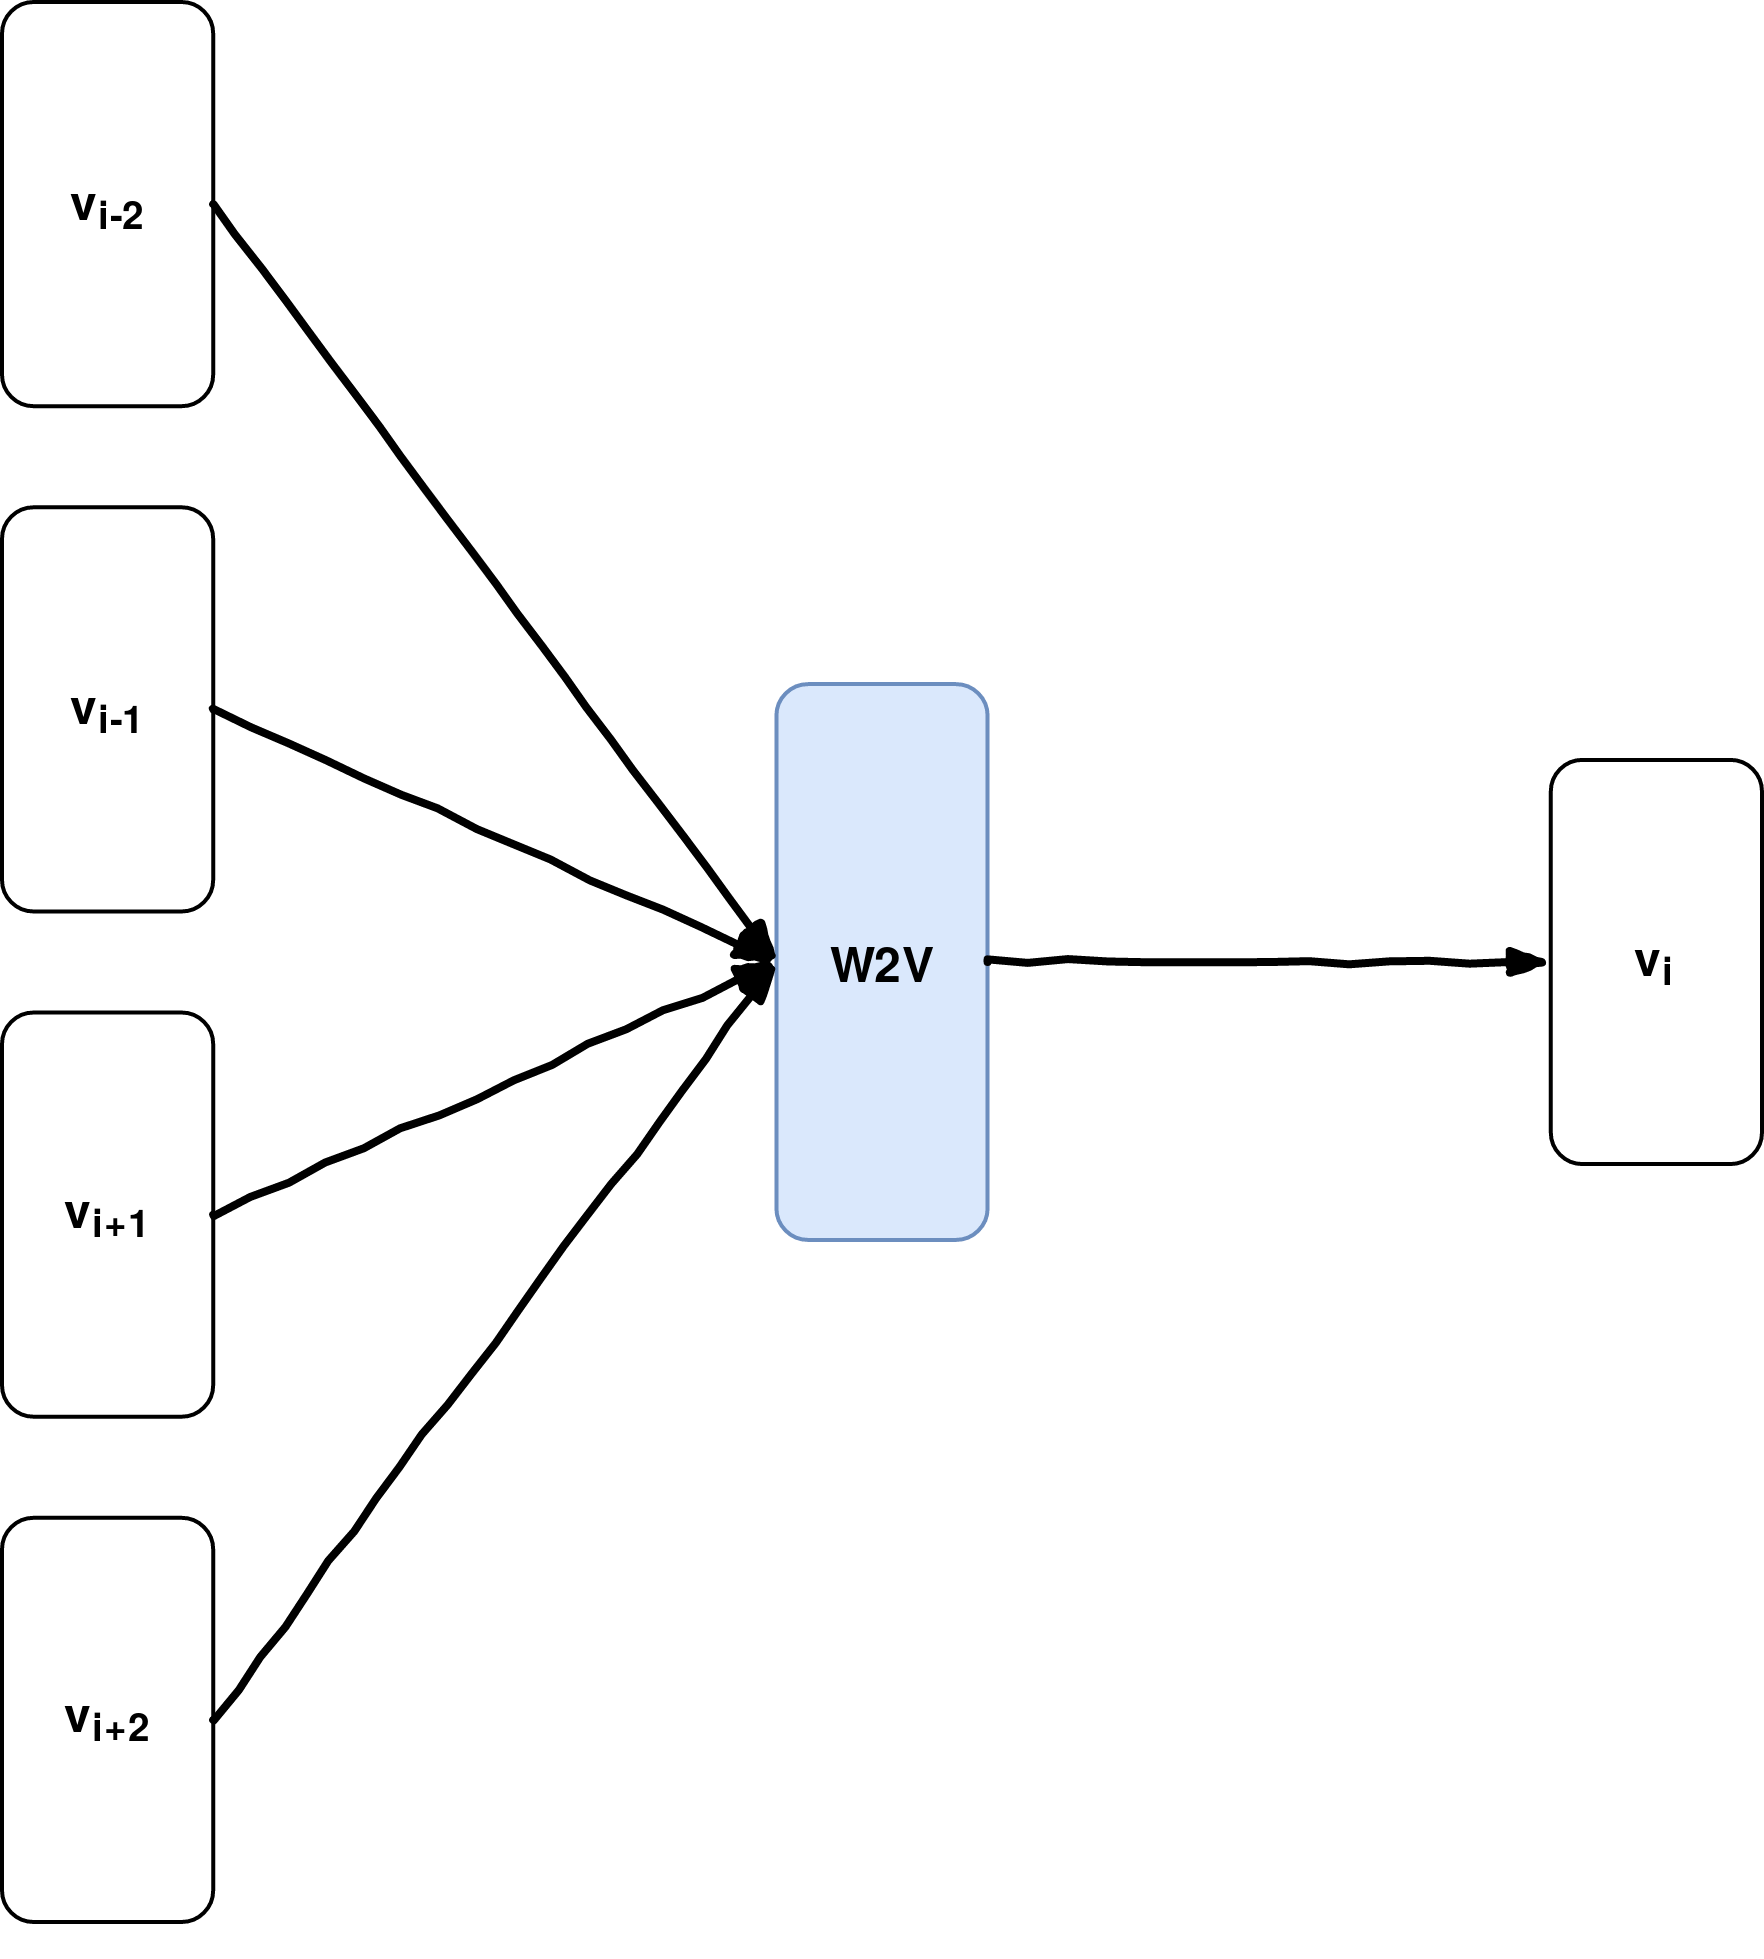
\includegraphics[width=0.5\textwidth,height=150px]{cbow}
	\caption{CBOW modell}
\end{figure}

Skip-Gram modell esetén pont az ellenkezője történik. A háló bemenete $v_i$
$\left( i \in \left|D\right| \right)$ vektor lesz. A tanítás célja, hogy a háló prediktálja az i. szó k méretű kontextusának one-hot kódolt vektorait ($v_{i-k},...,v_{i-1}, v_{i+1},..., v_{i+k} : k \in \mathbb{N}$), közben a háló a rejtett rétegében megtanulja a Word2Vec reprezentációt.

\begin{figure}[H]
	\centering
	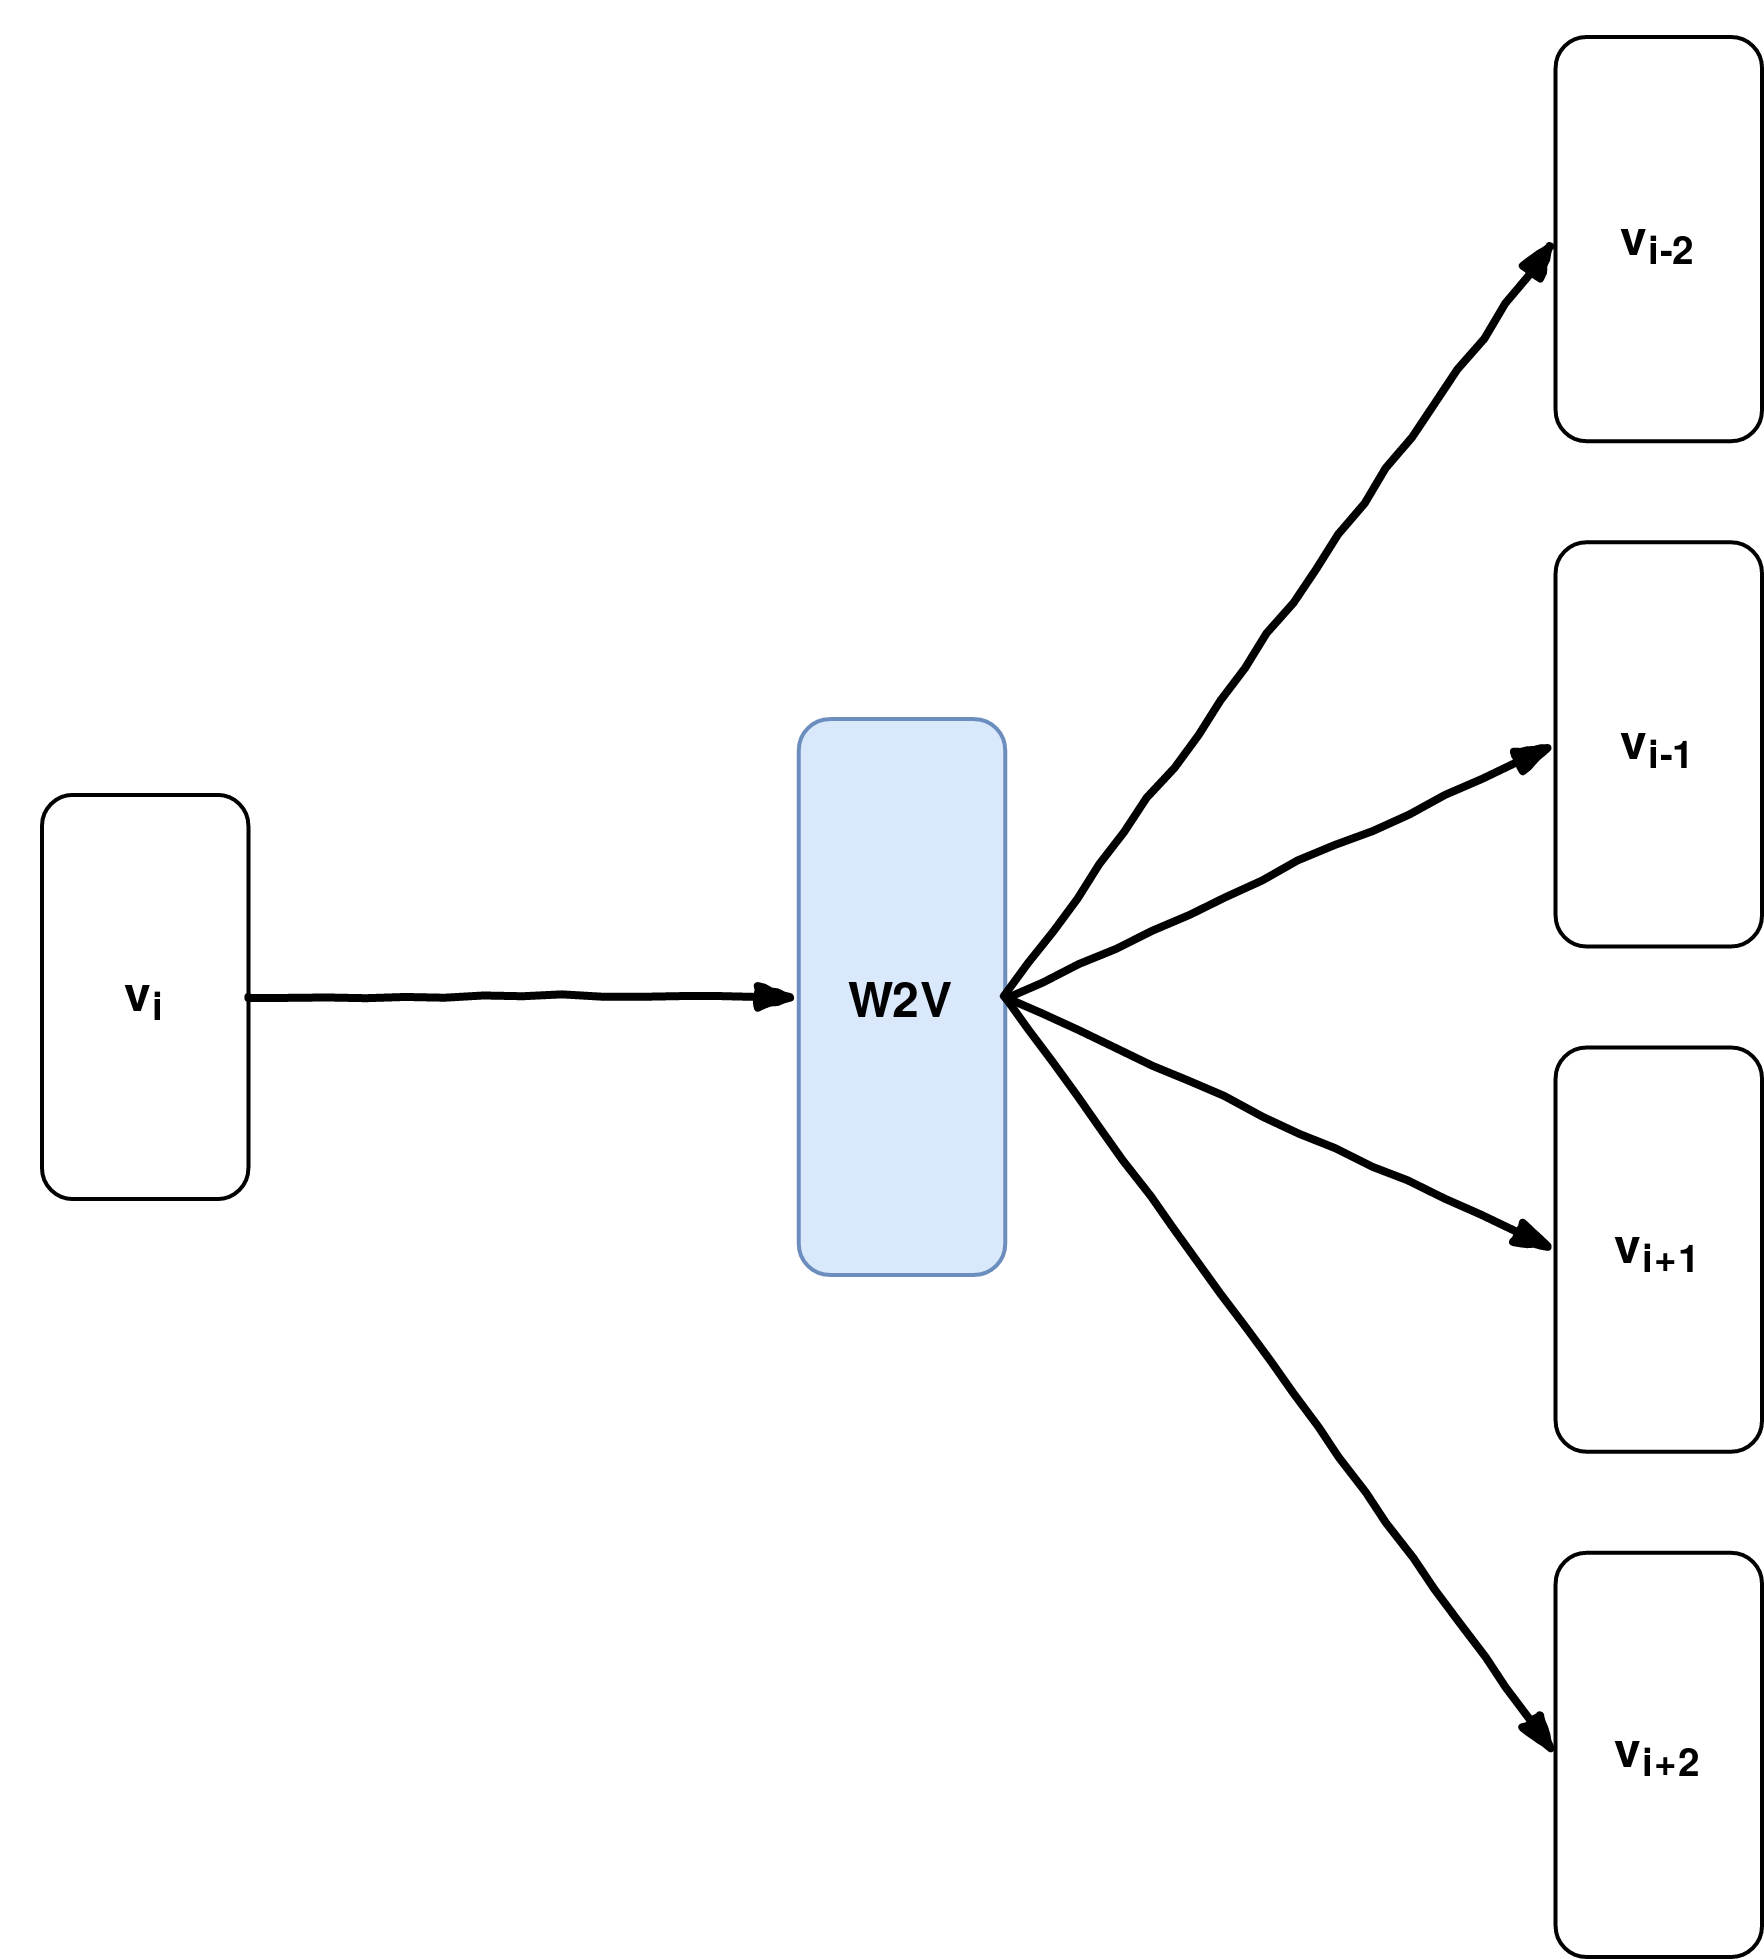
\includegraphics[width=0.5\textwidth,height=150px]{skip-gram}
	\caption{Skip-Gram modell}
\end{figure}

Egy jól tanított Word2Vec modell a hasonló jelentéstartalmú szóvektorokat közelre képezi egymáshoz a vektortérben. 
A teljesítmény növelése érdekében finomhangolhatjuk a tanítási paramétereket. Ilyen beavatkozás lehet ha növeljük a halmaz méretét, amellyel Word2Vec modellünket tanítjuk, vagy emeljük a kontextus ablak méretét és a reprezentációs dimenziót.

\begin{note}
	A Skip-Gram modell a ritka szavak, míg a CBOW modell a gyakori szavak esetén készít pontosabb reprezentációt.
\end{note}


\subsubsection{GloVe}
A Word2Vec bemutatását követő évben újabb nagy lépés történt a szóbeágyazás világában, a \textit{Stanford University} NLP kutatócsoportja publikálta a GloVe módszert.

A GloVe (\textit{Global Vectors}) \cite{pennington2014glove} reprezentációs módszer a Word2Vec-hez képest egy korpusz lokális statisztkáján kívül a globális statisztikáit is figyelembe veszi. 

\begin{definition}
	Adott egy korpusz, melynek elemszáma V. Az $X \in \mathbb{N}^{V \times V}$ mátrixot közös előfordulási mátrixnak nevezzük, ahol $X_{ij}$ az a szám, ahányszor i. szó kontextusában j. szó megjelenik.  
\end{definition}

A GloVe modell tanítása egy korpusz közös előfordulási mátrixának nemnulla elemein történik. A GloVe modell egy log-bilineáris modell, amely feladata, hogy kiszámítsa a következő szó valószínűségét azon kontextusa alapján.

A módszer mögötti intuíció az, hogy a közös előfordulási valószínűségek hányadosa értékes információval szolgálhat a leképezés során. Így a feladat célja, hogy a tanult szóvektorok skaláris szorzata megegyezzen a szavak közös előfordulási valószínűségének logaritmusával. Mivel $\log \left( \frac{A}{B} \right) = \log \left( A \right) - \log \left( B \right)$, így ez a cél összekapcsolja az előfordulási valószínűségek arányszámát a vektorok távolságával.

Ugyan a globális statisztikáknak köszönhetően a GloVe több feladatban is túlteljesíti a Word2Vec-et, a tanításához szükséges közös előfordulási mátrix memóriaigénye magas. Paraméterhangolás esetén újból fel kell építenie a mátrixot, mely költséges művelet.

\subsubsection{ELMo}
A Word2Vec és a GloVe már alkalmas szemantikus információ leképezésére, azonban esetükben az ellentétes szópárok közel kerülnek egymáshoz. Azon feladatoknál, melyeknél az ellentétes szavak kiemelt szerepűek – például a hangulatelemzés – limitációk jelentkezhetnek, továbbá ezen algoritmusok rosszul kezelik az ismeretlen szavakat is.

A Word2Vec és a GloVe csak szavankénti kontextusfüggetlen reprezentáció tanulására képes. Ez azt jelenti, hogy a szótárban található szavakhoz bijektív módon hozzárendelnek egy vektort, így nem számít az adott szó szövegkörnyezete, amelyre alkalmazzák. Az Embeddings from Language Models (ELMo) \cite{elmo} figyelembe veszi a lexémák kontextusát, mondaton belüli elhelyezkedését is, továbbá használat közben állítja elő a vektorokat.

A modell tanításához használt neurális háló több réteg kétirányú LSTM (biLSTM) konkatenációja. A különböző rétegek más és más típusú információt képesek eltárolni.

\begin{figure}[H]
	\centering
	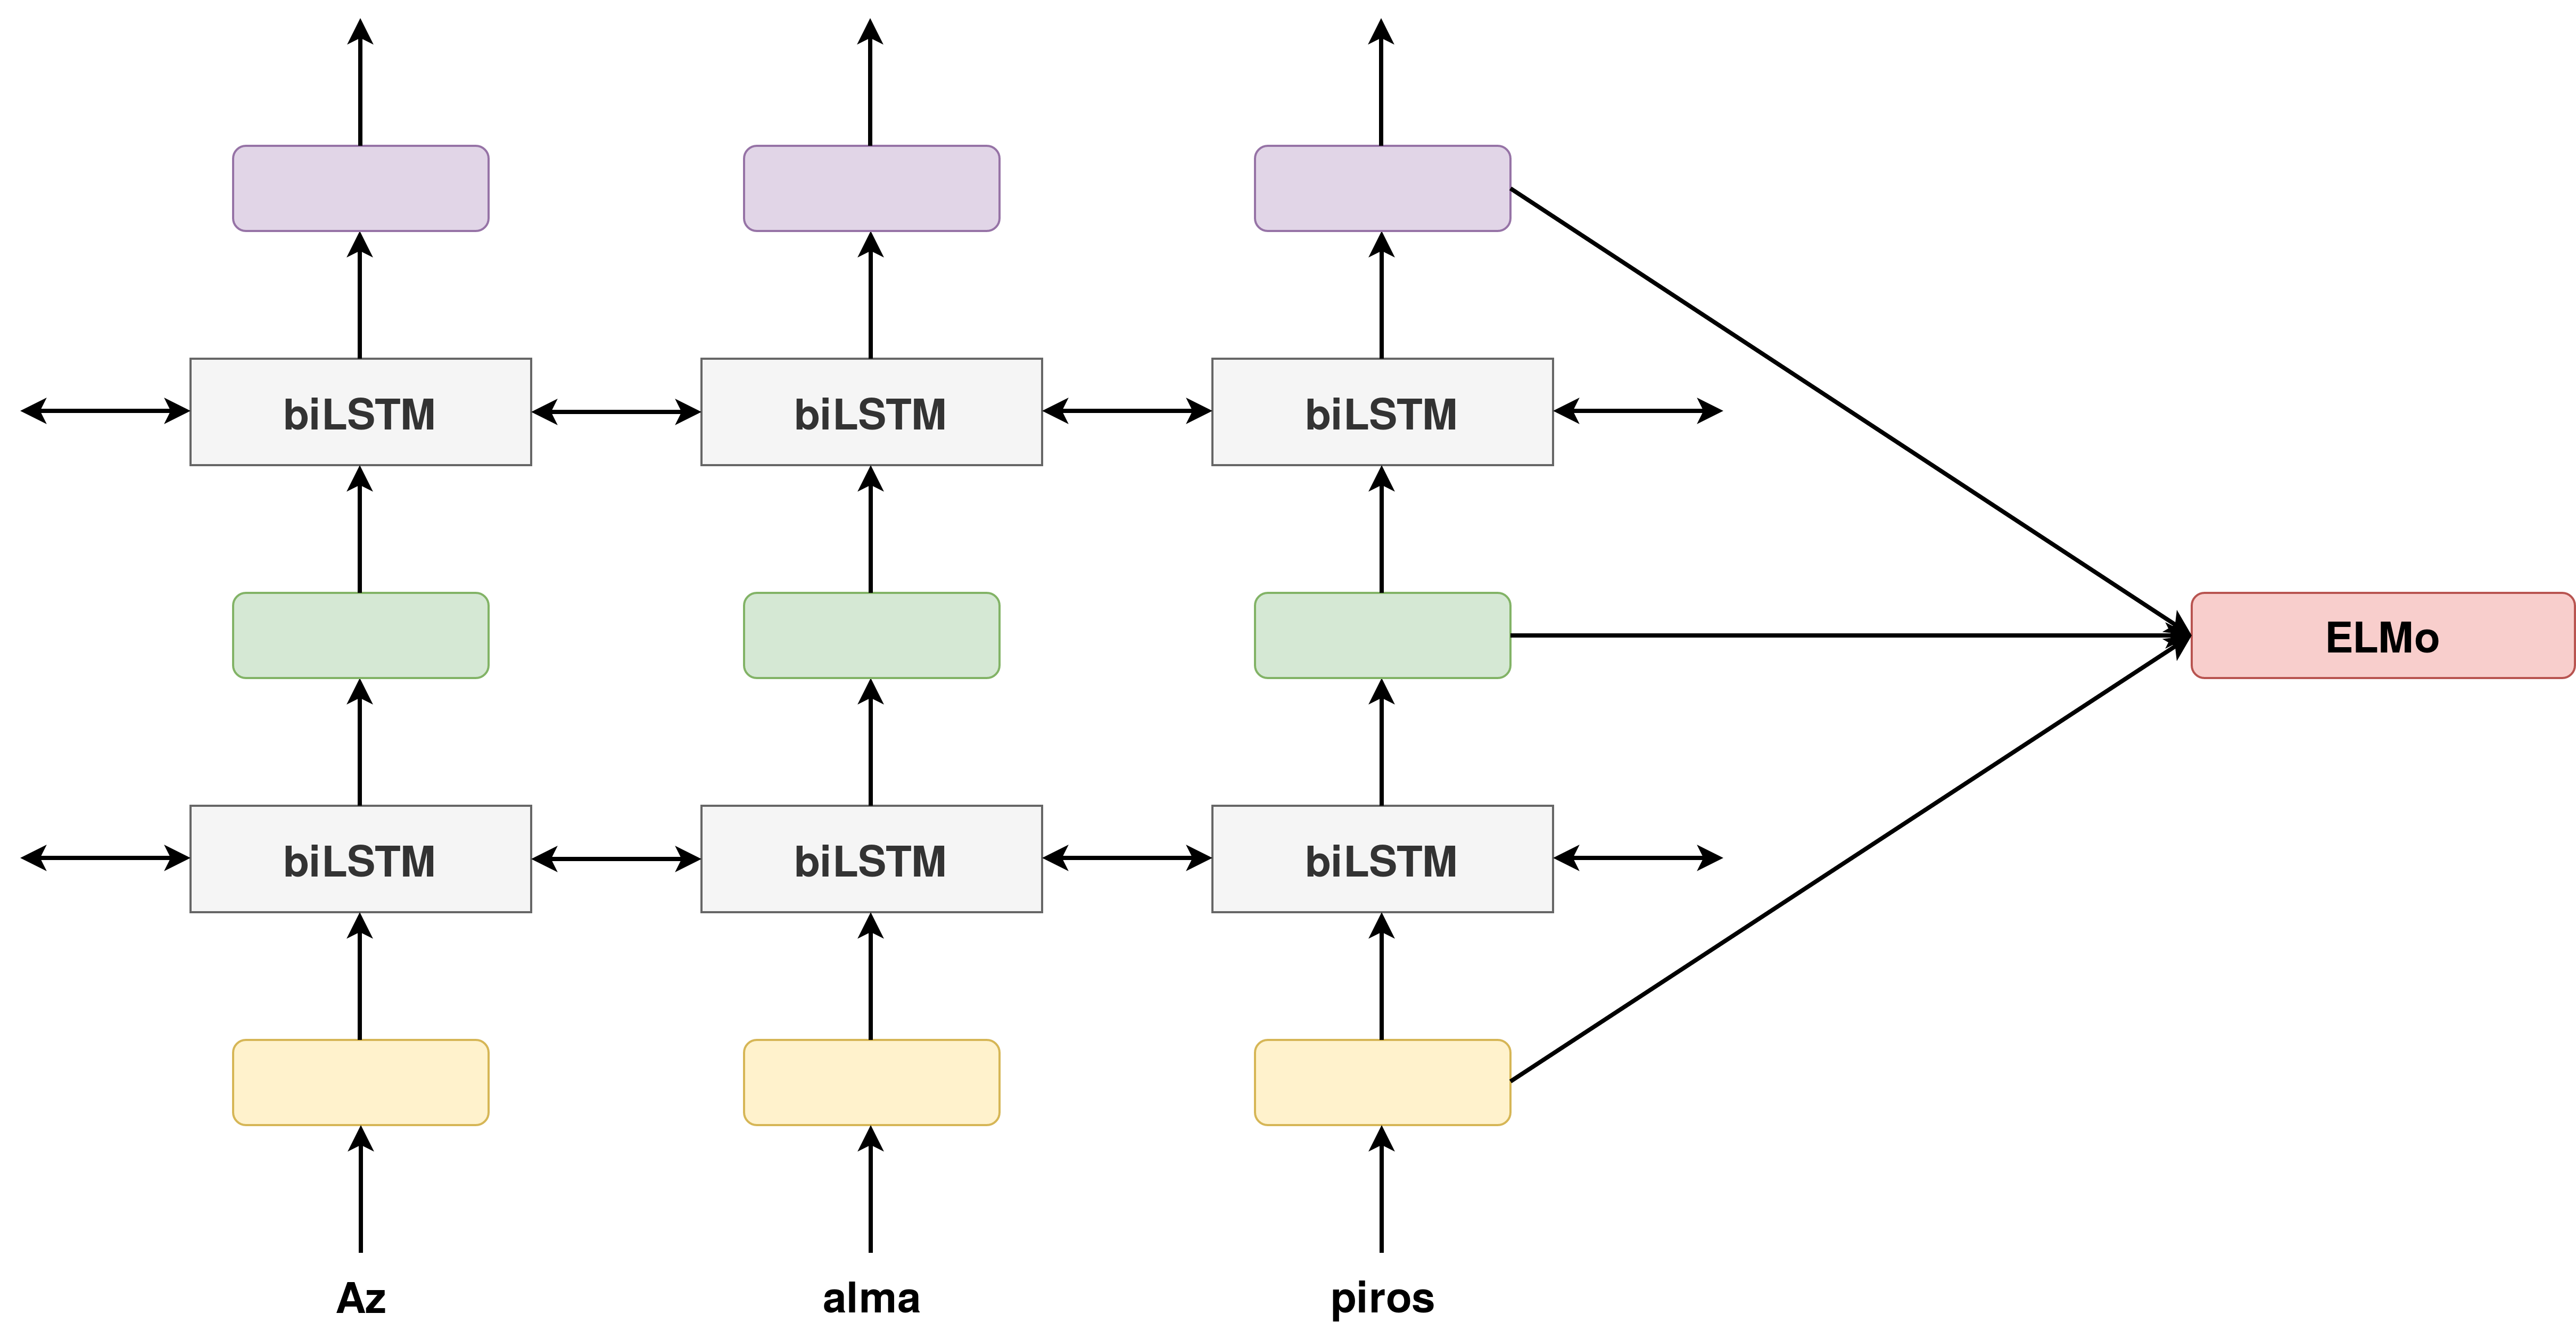
\includegraphics[width=0.8\textwidth,height=200px]{ELMo}
	\caption{ELMo modell}
\end{figure}

Az ELMo a különböző rétegek kimenetének feladatspecifikus kombinációján alapszik. Egy adott NLP feladatra minden BiLSTM réteg egyedi súlyt kap. A végső háló 2 darab BiLSTM rétegből áll, minden LSTM réteg 4096 széles.
Az így kapott sekély kétirányú módszer jelentősen javított a szóvektorok pontosságán.

Bár az ELMo egy karakter (konkatenáció) alapú reprezentációs algoritmus, szavakat ábrázol. Ezen tulajdonsága alapján képes kezelni az addig nem látott szavak problémáját is.


\subsubsection{BERT}
Egy 2018-ban publikált cikk \cite{char} rámutatott arra, hogy a karakteralapú algoritmusok – tehát amelyek karaktereket fogadnak bemenetül tanulás során – nem teljesítenek olyan jól, mint a szóalapú társaik. A Bidirectional Encoder Representations from Transformers (BERT) \cite{2018arXiv181004805D} egy a Google által kifejlesztett transformer architektúrájú nyelvi modell. Az ELMo-hoz hasonlóan ez is kétirányú, azaz egy szó mindkét oldali kontextusát figyelembe veszi a tanulás alatt. A BERT azonban bemenetként nem szavakat és nem is karaktereket kap, hanem szótöredékeket.

A tanítást a \textit{transfer learning} szerint két fázisra bontották: előtanítás és finomhangolás. 

Az előtanítás két feladatból állt: \textit{következő mondat} és \textit{maszkolás}.
A bemenetben megadták a szótöredék token-eket, a token-ekhez tartozó mondaton belüli helyadatokat és azt, hogy az adott token A vagy B mondat közül melyikhez tartozik.

\begin{figure}[H]
	\centering
	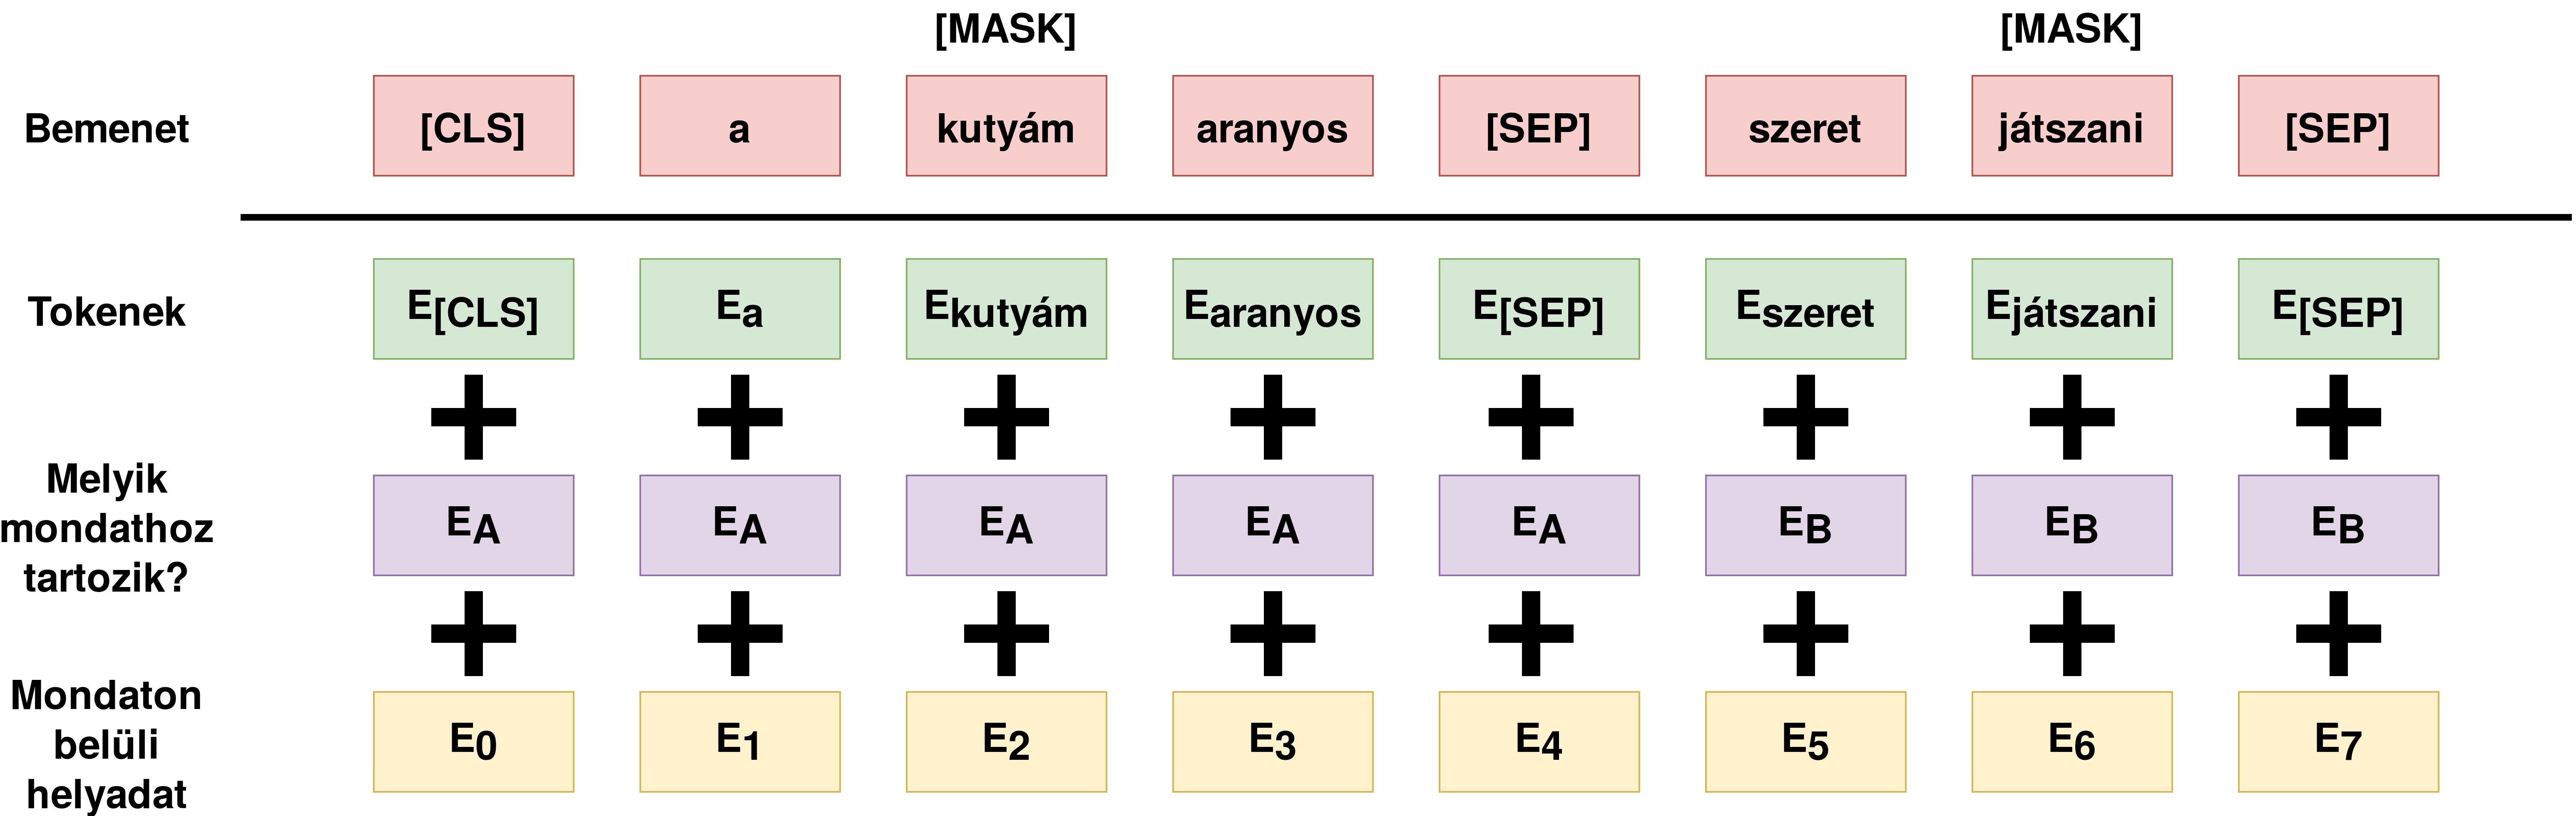
\includegraphics[width=1\textwidth,height=180px]{BERT}
	\caption{A BERT bemenete}
\end{figure}

 A \textit{következő mondat} esetében a mélyháló feladata kitalálni, hogy A[SEP]B input mondatokra B rákövetkezője-e A-nak. A \textit{maszkolás} során véletlenszerűen letakarták a token-eket a mondatokban és a mélyháló megpróbálta kitalálni, hogy eredetileg melyik szó volt a [MASK] token helyén.  A [CLS] token a klasszifikációs feladat alatt a mondatot ábrázolja, a [SEP] a mondatok közötti szeparátor és a [MASK] a letakart szótöredékeket helyettesíti.

A továbbiakban a modell finomhangolása az adott NLP feladat szerint történik.

Míg az ELMo különböző balról-jobbra és jobbról-balra olvasó rétegek konkatenációjaként állítja elő a vektorokat, addig a BERT a valódi mély architektúrájával csak egyszer dolgozza fel a token-eket. A \textit{transformer} architektúra nem igényel vektoriális bemenetet, saját reprezentációt épít a token-ek számára is.

A BERT szótöredék alapú megoldása egyesíti a karakteralapú modellek előnyét a szóalapú modellek előnyével. Képes kezelni az ismeretlen szavakat és performanciája mégis magas marad. A \textit{következő mondat} feladat a szövegben található mondatok közötti relációk, a \textit{maszkolás} pedig a mondatokon belüli szemantikai és szintaktikai információ ábrázolását segíti. Több NLP feladat megoldásában is jelenleg a BERT a \textit{State-of-the-art}.

\section{Reprezentáció a mondatok és magasabb nyelvi elemek szintjén}

Ahogy a lexémák szemantikai tartalmát sem határozza meg az őket alkotó karakterek lánca, úgy a mondatok sem értelmezhetőek pusztán a magukban foglalt szavak halmaza alapján. A mondatok és magasabb nyelvi elemek interpretálása során fontos tényezők lehetnek a bennük lévő szintaktikai viszonyok és a kontextus is.

Néhány NLP feladatnál, mint például a dokumentumok szemantikus keresésénél, vagy szöveg összegzésnél szükség lehet magasabb szintű reprezentációkra.  Ezek a módszerek szavak helyett mondatokat, bekezdéseket, vagy akár egész dokumentumokat tesznek numerikusan értelmezhetővé. 

\subsection{Mondatvektorok}
A szóvektorokhoz hasonlóan úgy kaphatunk mondatvektorokat, ha mondatokat helyezünk el egy vektortérbe. A tanítás során azonban a sorrendiség, az egyes lexémák változó súlya és a szintaktikai viszonyok megnehezíthetik dolgunkat. Szükség van egy technikára, mely segítségével leképezhetjük és szemantikai tartalmuknál fogva összegezhetjük a megfelelő rendezett szóvektorok sorozatát, így hozzájutva az adott mondat reprezentációjához. A módszerünk akkor hatékony, ha az azonos jelentéstartalmú mondatvektorok klaszterekbe tömörülnek a vektortérben.

\subsubsection{Skip-thought vektorok}
A Skip-though \cite{skip} egy 2015-ben bemutatott mondatreprezentációs módszer – a Skip-Gram algoritmus kiterjesztése – , amely a környező mondatokat is figyelembe veszi a tanulás során. 

A szerzők rekurrens enkóder-dekóder architektúrát használtak a tanításhoz. A neurális háló bemenete mondathármasok szavainak Word2Vec vektoraiból állt. A háló feladata $s_i$ mondat esetén $s_{i-1}$ és $s_{i+1}$ mondatok generálása volt.

\begin{figure}[H]
	\centering
	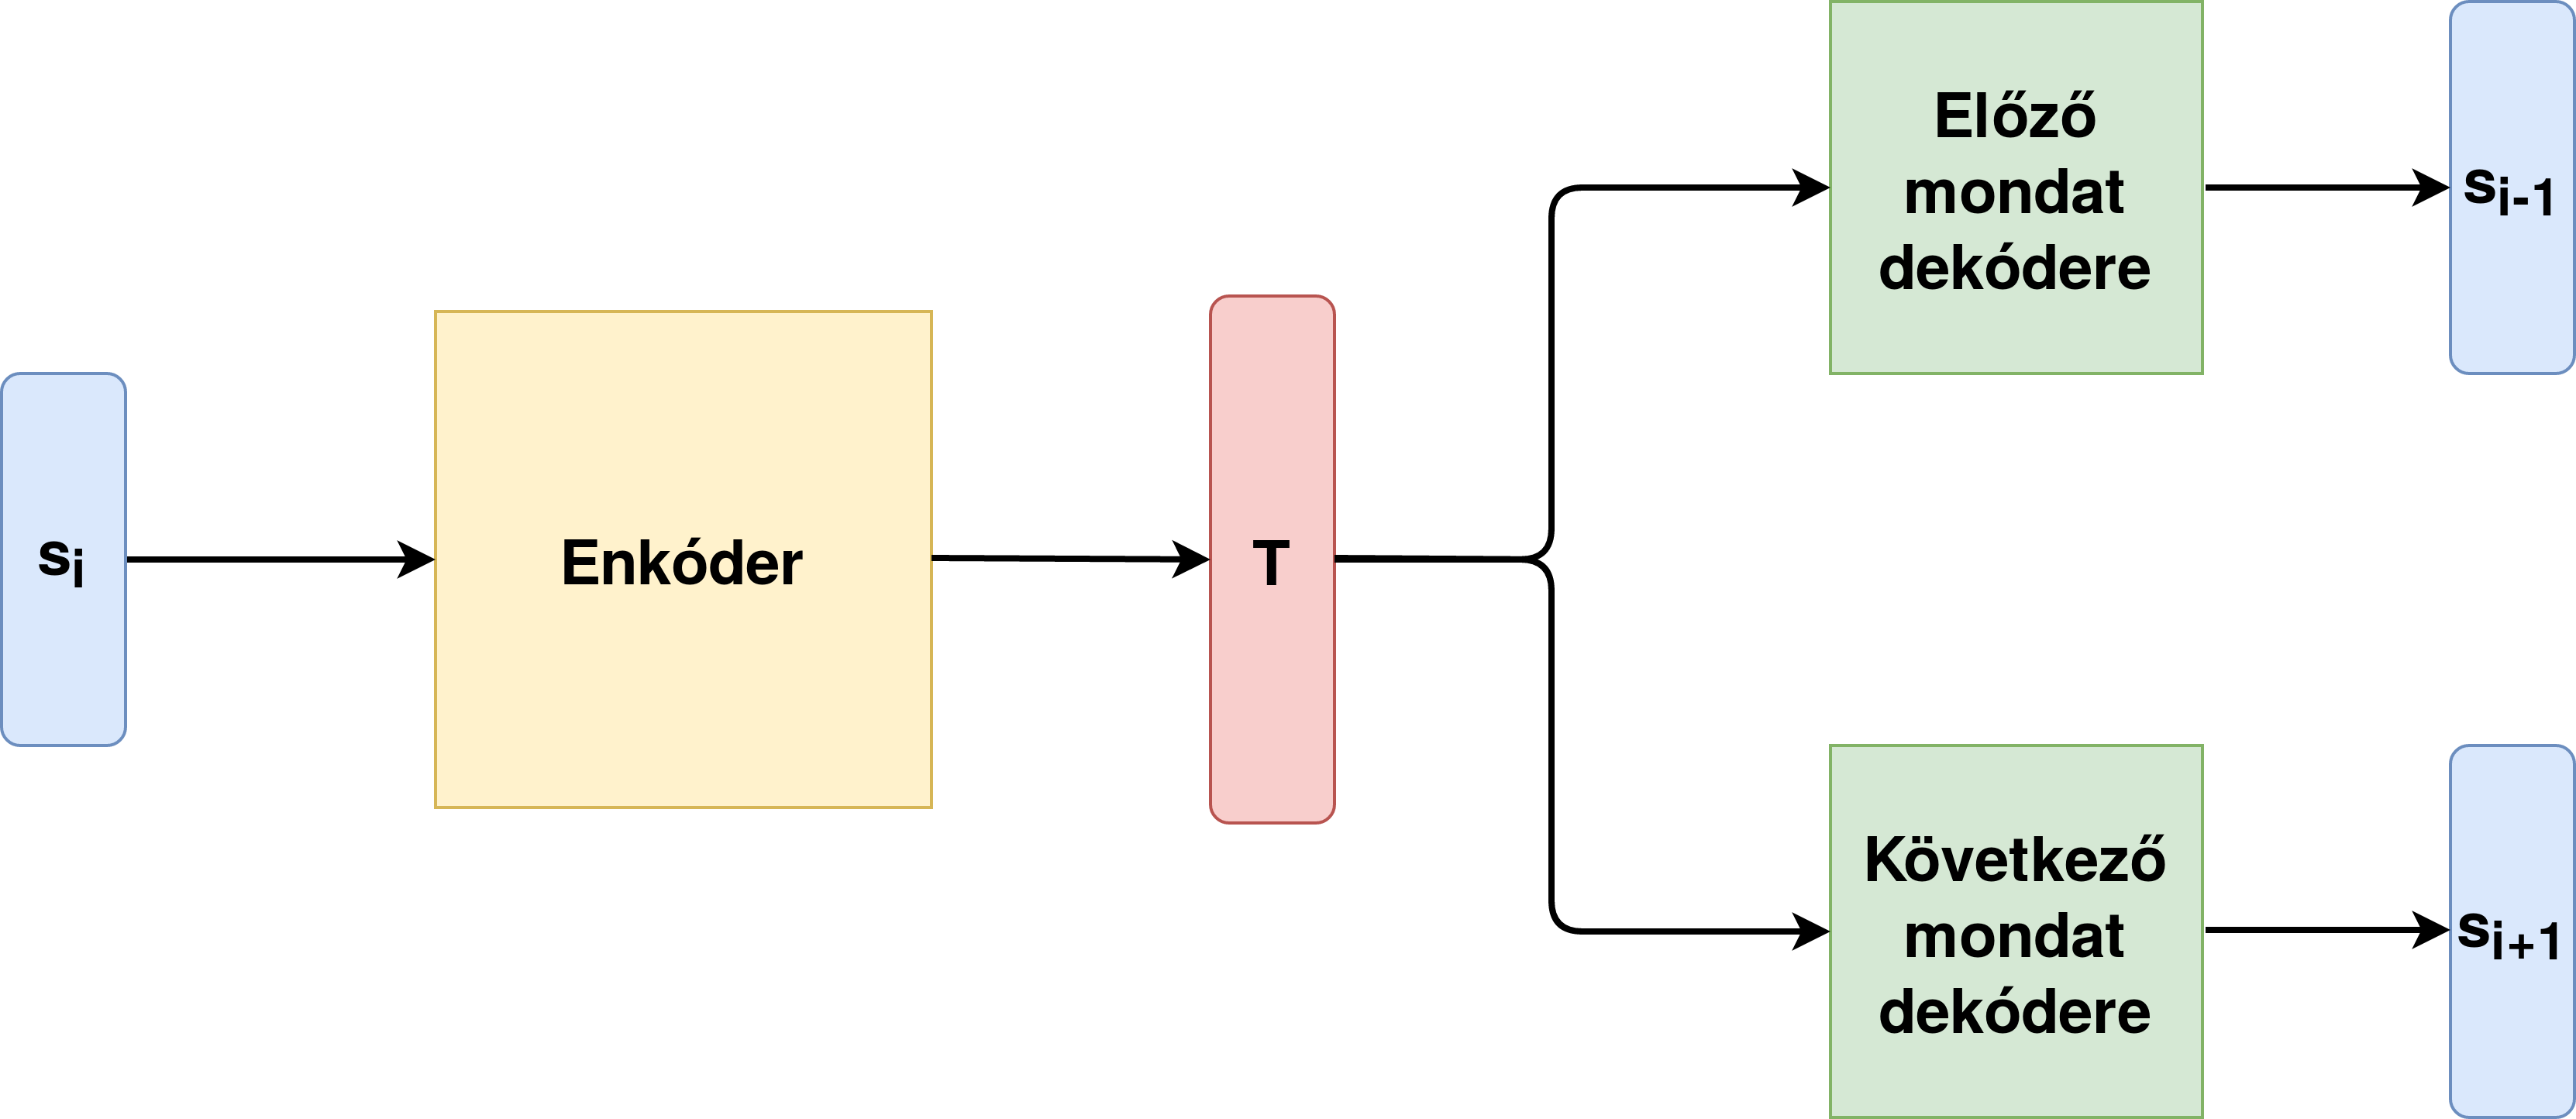
\includegraphics[width=0.6\textwidth,height=130px]{Skip-thought}
	\caption{A Skip-thought enkóder-dekóder architektúrája}
\end{figure}

Az enkóder és dekóder blokkokhoz rekurrens hálót használtak, melyek lehetnek LSTM és GRU rétegek is. Az enkóder célja a legjobb teljesítményével segíteni a dekóder blokkokat, míg a dekóder blokkok célja minimalizálni az előző és a következő mondat rekonstrukciós hibáját. Olyan szavak esetén, melyeket a háló még nem ismer, tanítottak egy $f:V_{w2v} \rightarrow V_{rnn}$ lineáris leképezést, ahol $V_{w2v}$ és $V_{rnn}$ rendre a Word2Vec és a rekurrens modell szótára. A reprezentáció vektora a rejtett, úgy nevezett \textit{thought} vektor (T).

Bár a \textit{Skip-thought} módszer képes a mondaton belüli és kívüli sorrendiségi információ leképezésére is, csak olyan esetben teljesít megfelelően, ahol az egyes mondatok – melyekre alkalmazzák – megfelelő kontextusban szerepelnek, nem izoláltak.

\subsubsection{InferSent}
2017-ben a Facebook kutatói jelentős áttörést értek el a mondatszintű reprezentációs módszerek terén, a technika neve InferSent \cite{infer}. Hasonló algoritmusokkal ellentétben a szerzők felügyelt tanítást végeztek, melyhez az SNLI adathalmazt vették igénybe. A cikk megmutatta, hogy egy kisebb adathalmazon történő felügyelt tanítás felülmúlhatja a nagyobb adathalmazon nem felügyelt módon tanított modellek teljesítményét.

Az SNLI adathalmaz 570 ezer darab – ember által írt és címkézett – mondatpárból áll. A címkék a következők: következmény, ellentmondás és semleges.

Négyféle neurális architektúrát összemérve a legpontosabb eredményt a BiLSTM + max pooling mutatta. 

\begin{figure}[H]
	\centering
	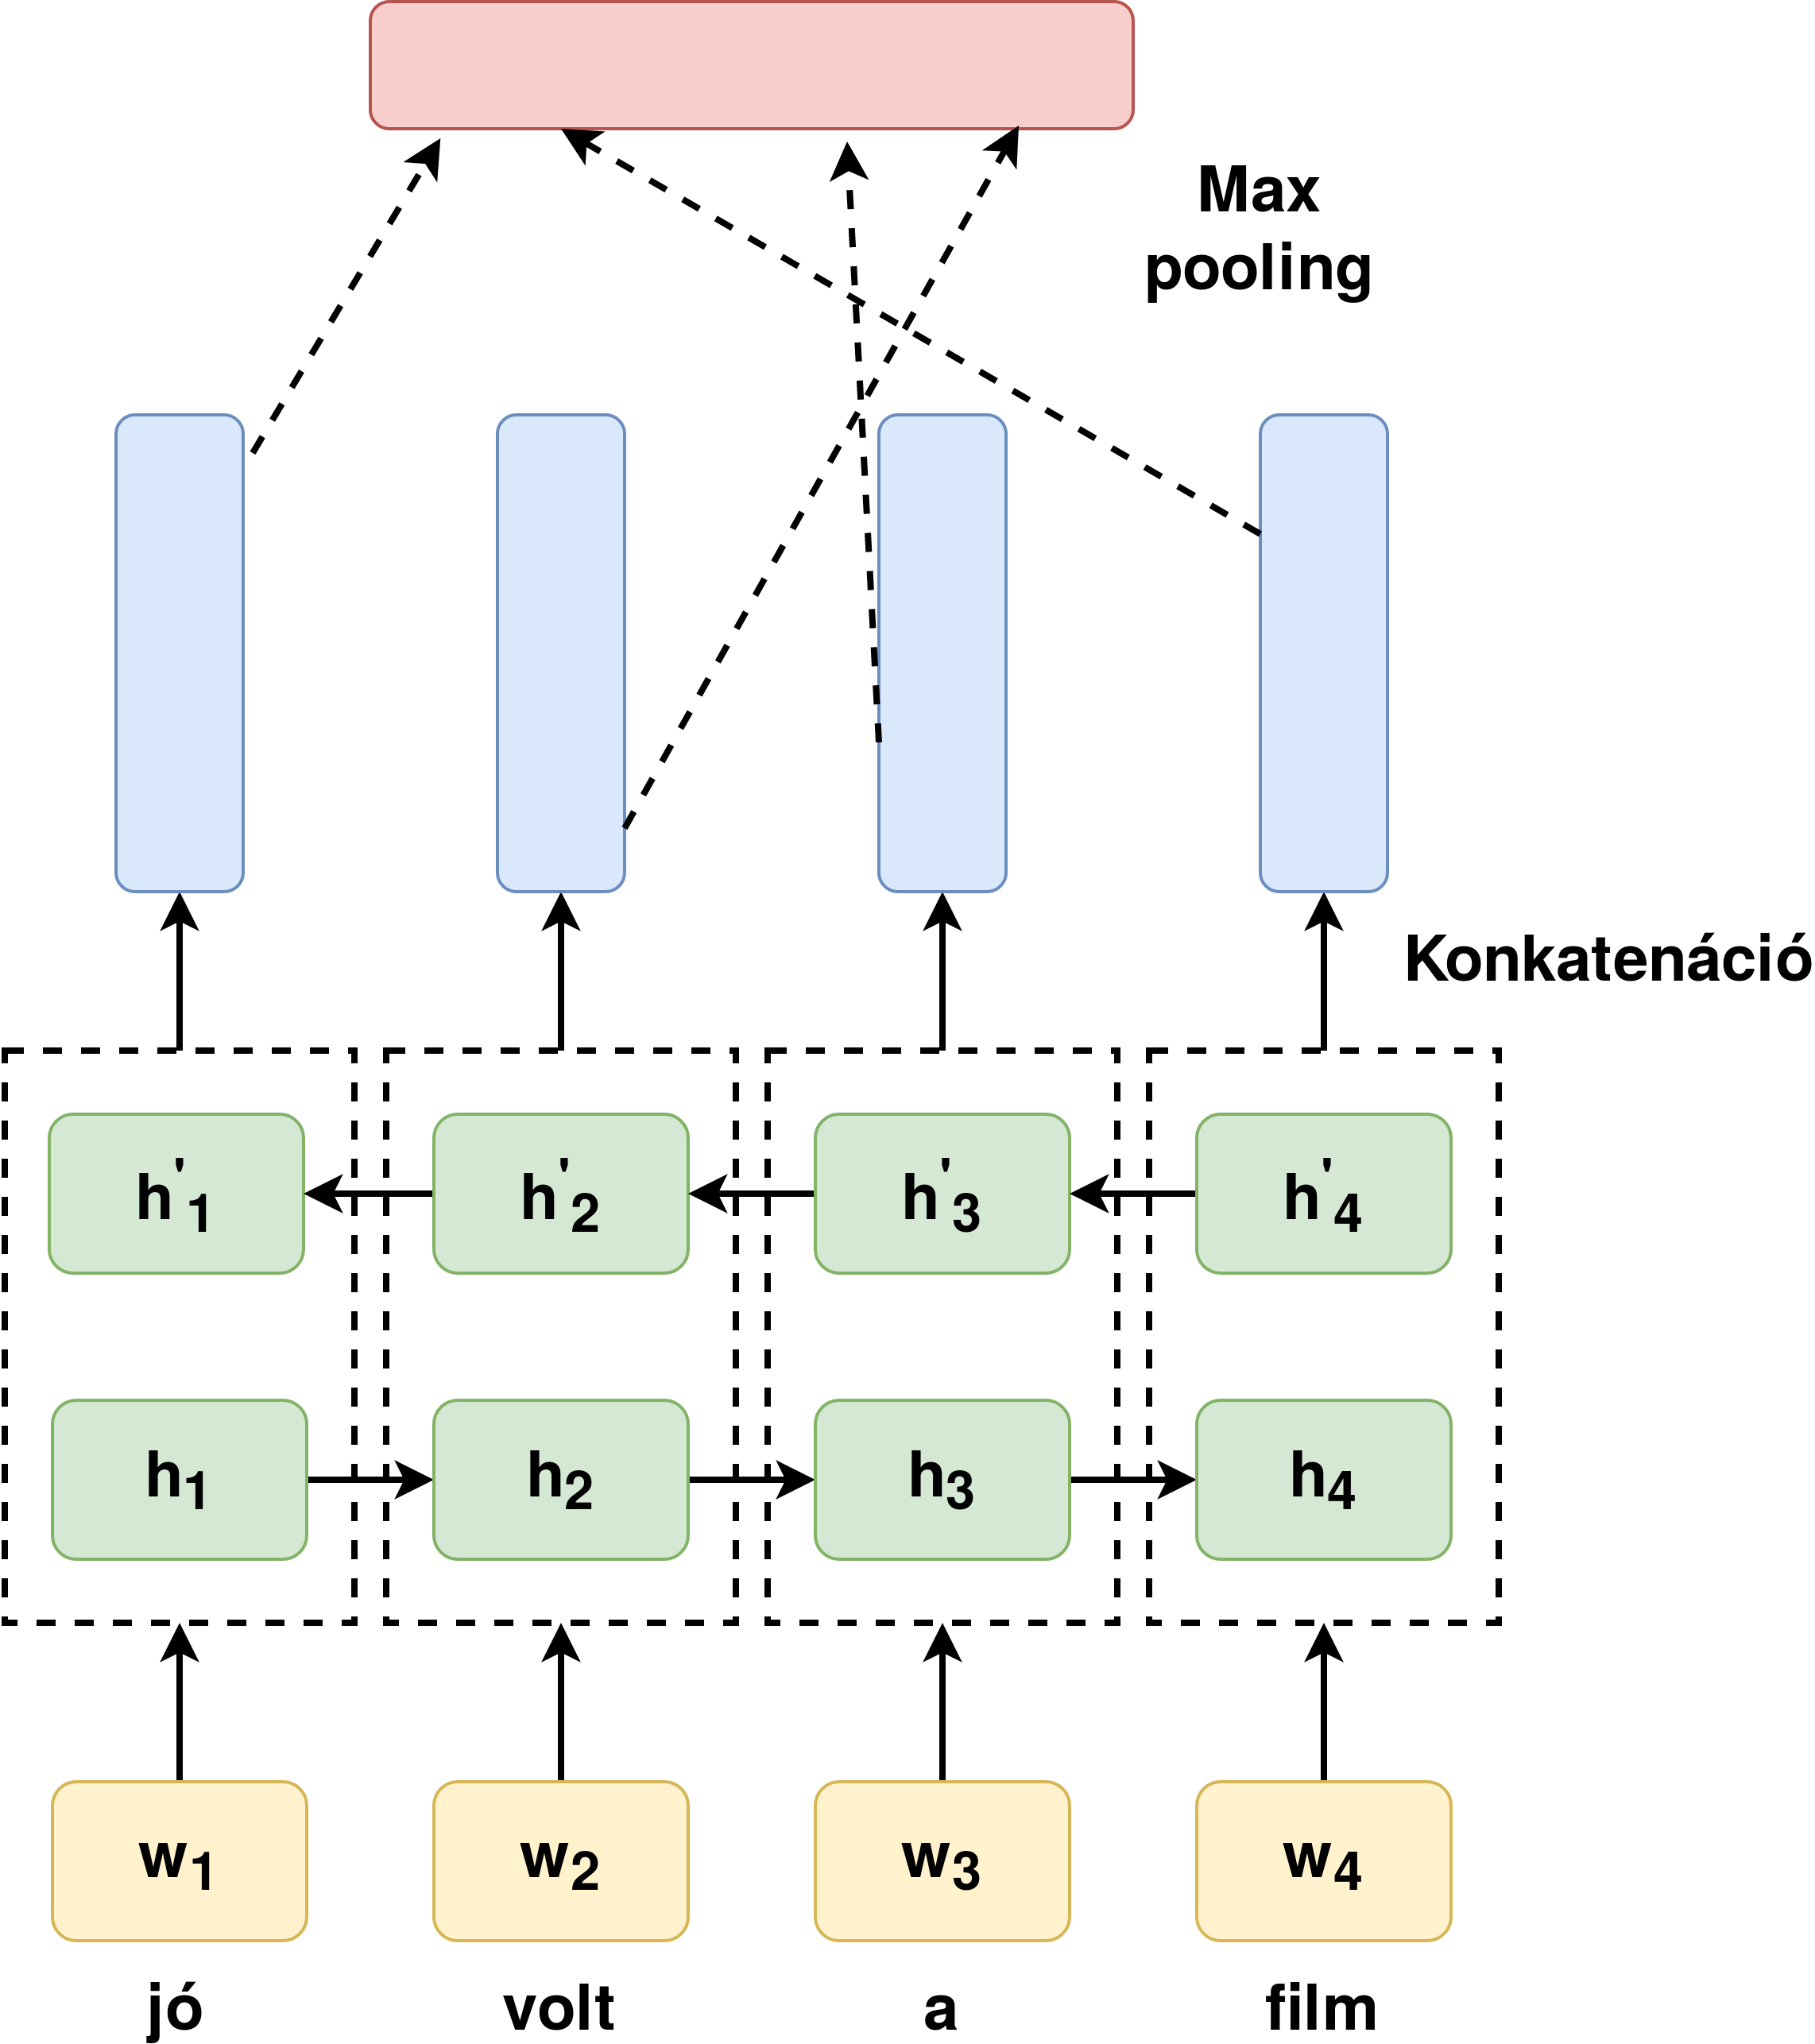
\includegraphics[width=0.5\textwidth,height=200px]{biLSTM-max-pooling}
	\caption{A BiLSTM + max pooling architektúra}
\end{figure}

Az SNLI feldolgozásához szükséges NLI feladat speciális szerkezetet igényel. Mivel kontextusfüggetlen reprezentációt akartak előállítani, amely izolált formában is működik, a mondatpárok GloVe vektorait szeparáltan enkódolták.

\begin{figure}[H]
	\centering
	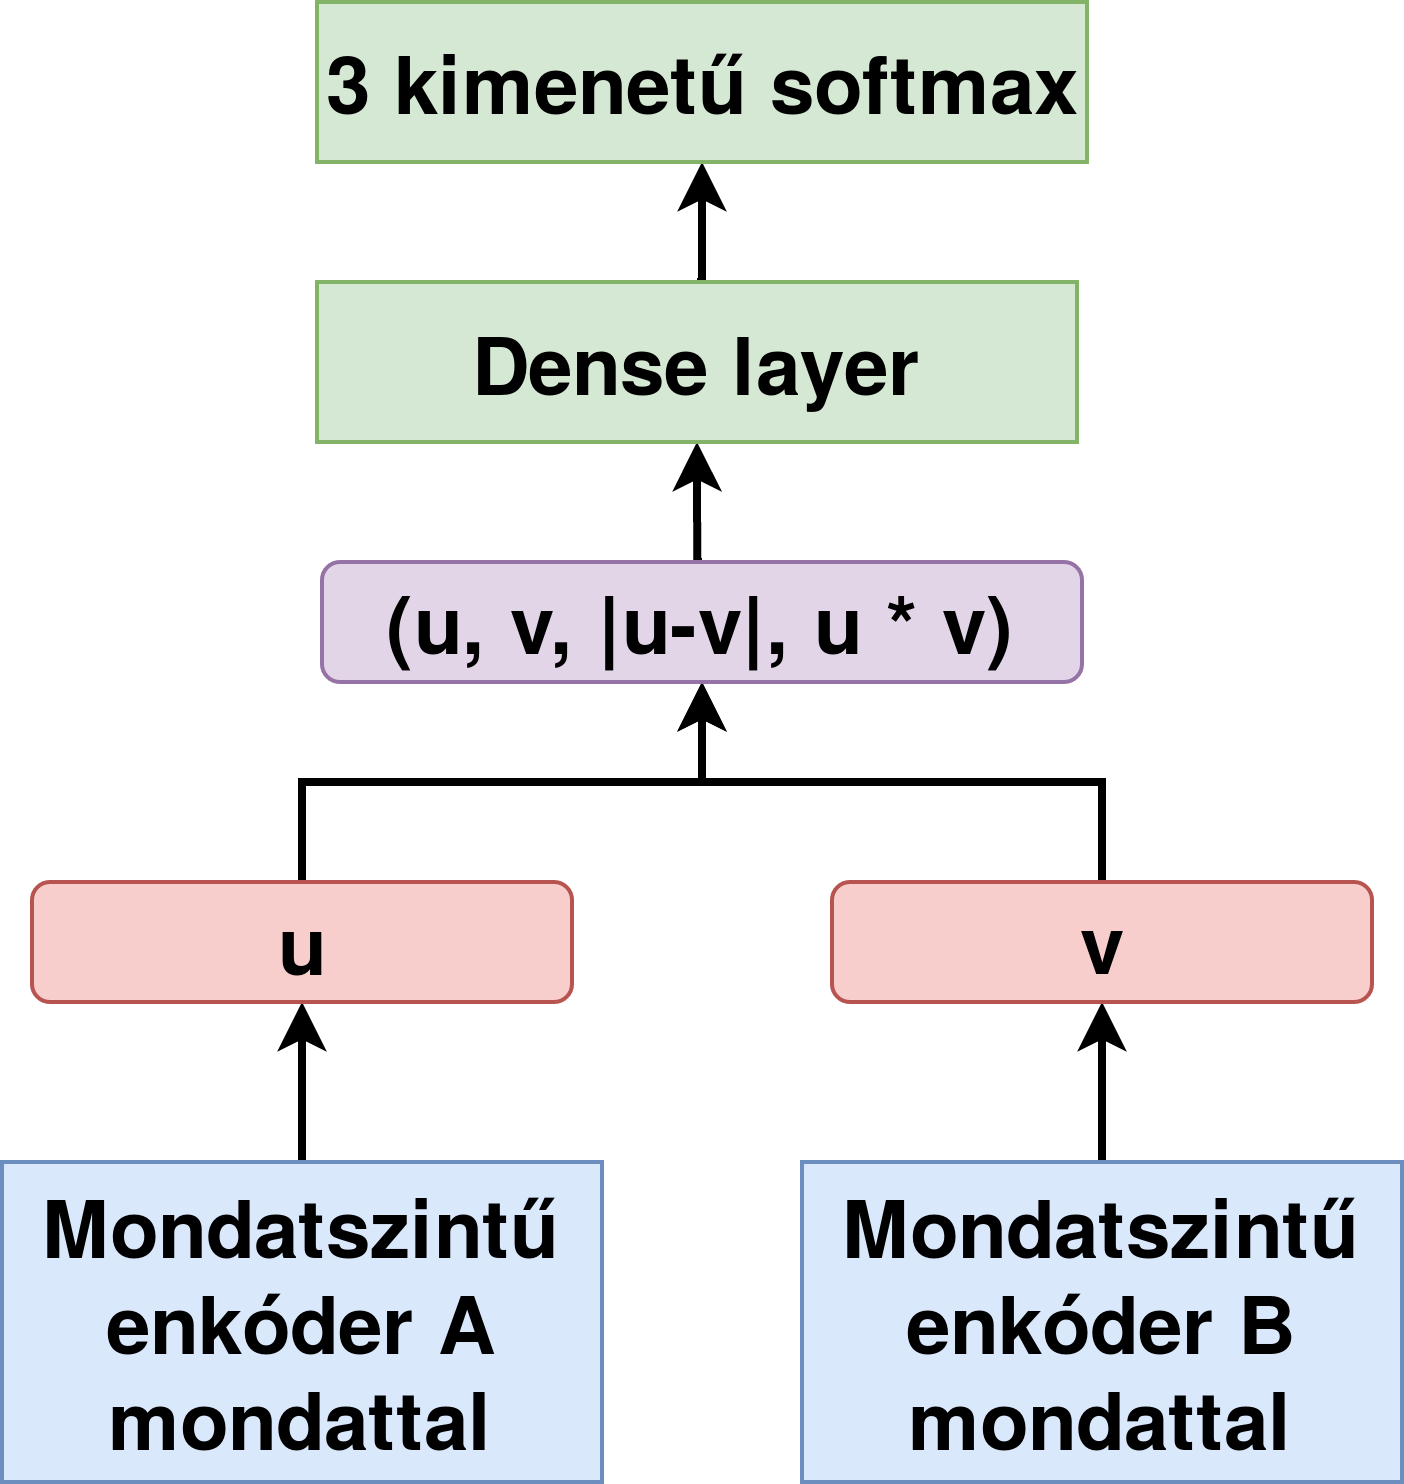
\includegraphics[width=0.5\textwidth,height=150px]{NLI}
	\caption{Az NLI feladat}
\end{figure}

Az így készült u és v vektorokból egy speciális reprezentáció készült: u, v, $\left| u - v \right|$ és $u \ast v$ (vektoriális szorzat) konkatenációjával, melyet végül egy 3 osztályú klasszifikáló hálóba vezettek.

A szerzők a reprezentációs vektorméret növelésével pontosabb eredményt kaptak, de a vektorok memóriaigénye emelkedett. Az InferSent megoldja a kontextusfüggőség problémáját, így a módszer már szövegrészletekre is alkalmazható.

\begin{note}
	Az InferSent napjaink egyik legjobb teljesítményű szemantikus reprezentációs algoritmusa.
\end{note}

\subsubsection{USE}
Az InferSent bemutatását követő évben a Google Research csapata a modern reprezentációs módszereket vizsgálta a \textit{transfer learning} aspektusából. A Universal Sentence Encoder (USE) \cite{use} egy mondatszintű  algoritmus, mely célja, hogy a használója könnyedén igényeire tudja formálni, annak érdekében, hogy pontosabb leképezést kapjon. A szerzők két architektúrát használtak: a BERT-ben említett \textit{transformer}-t és a DAN-t (\textit{Deep Averaging Network}). 

\begin{figure}[H]
	\centering
	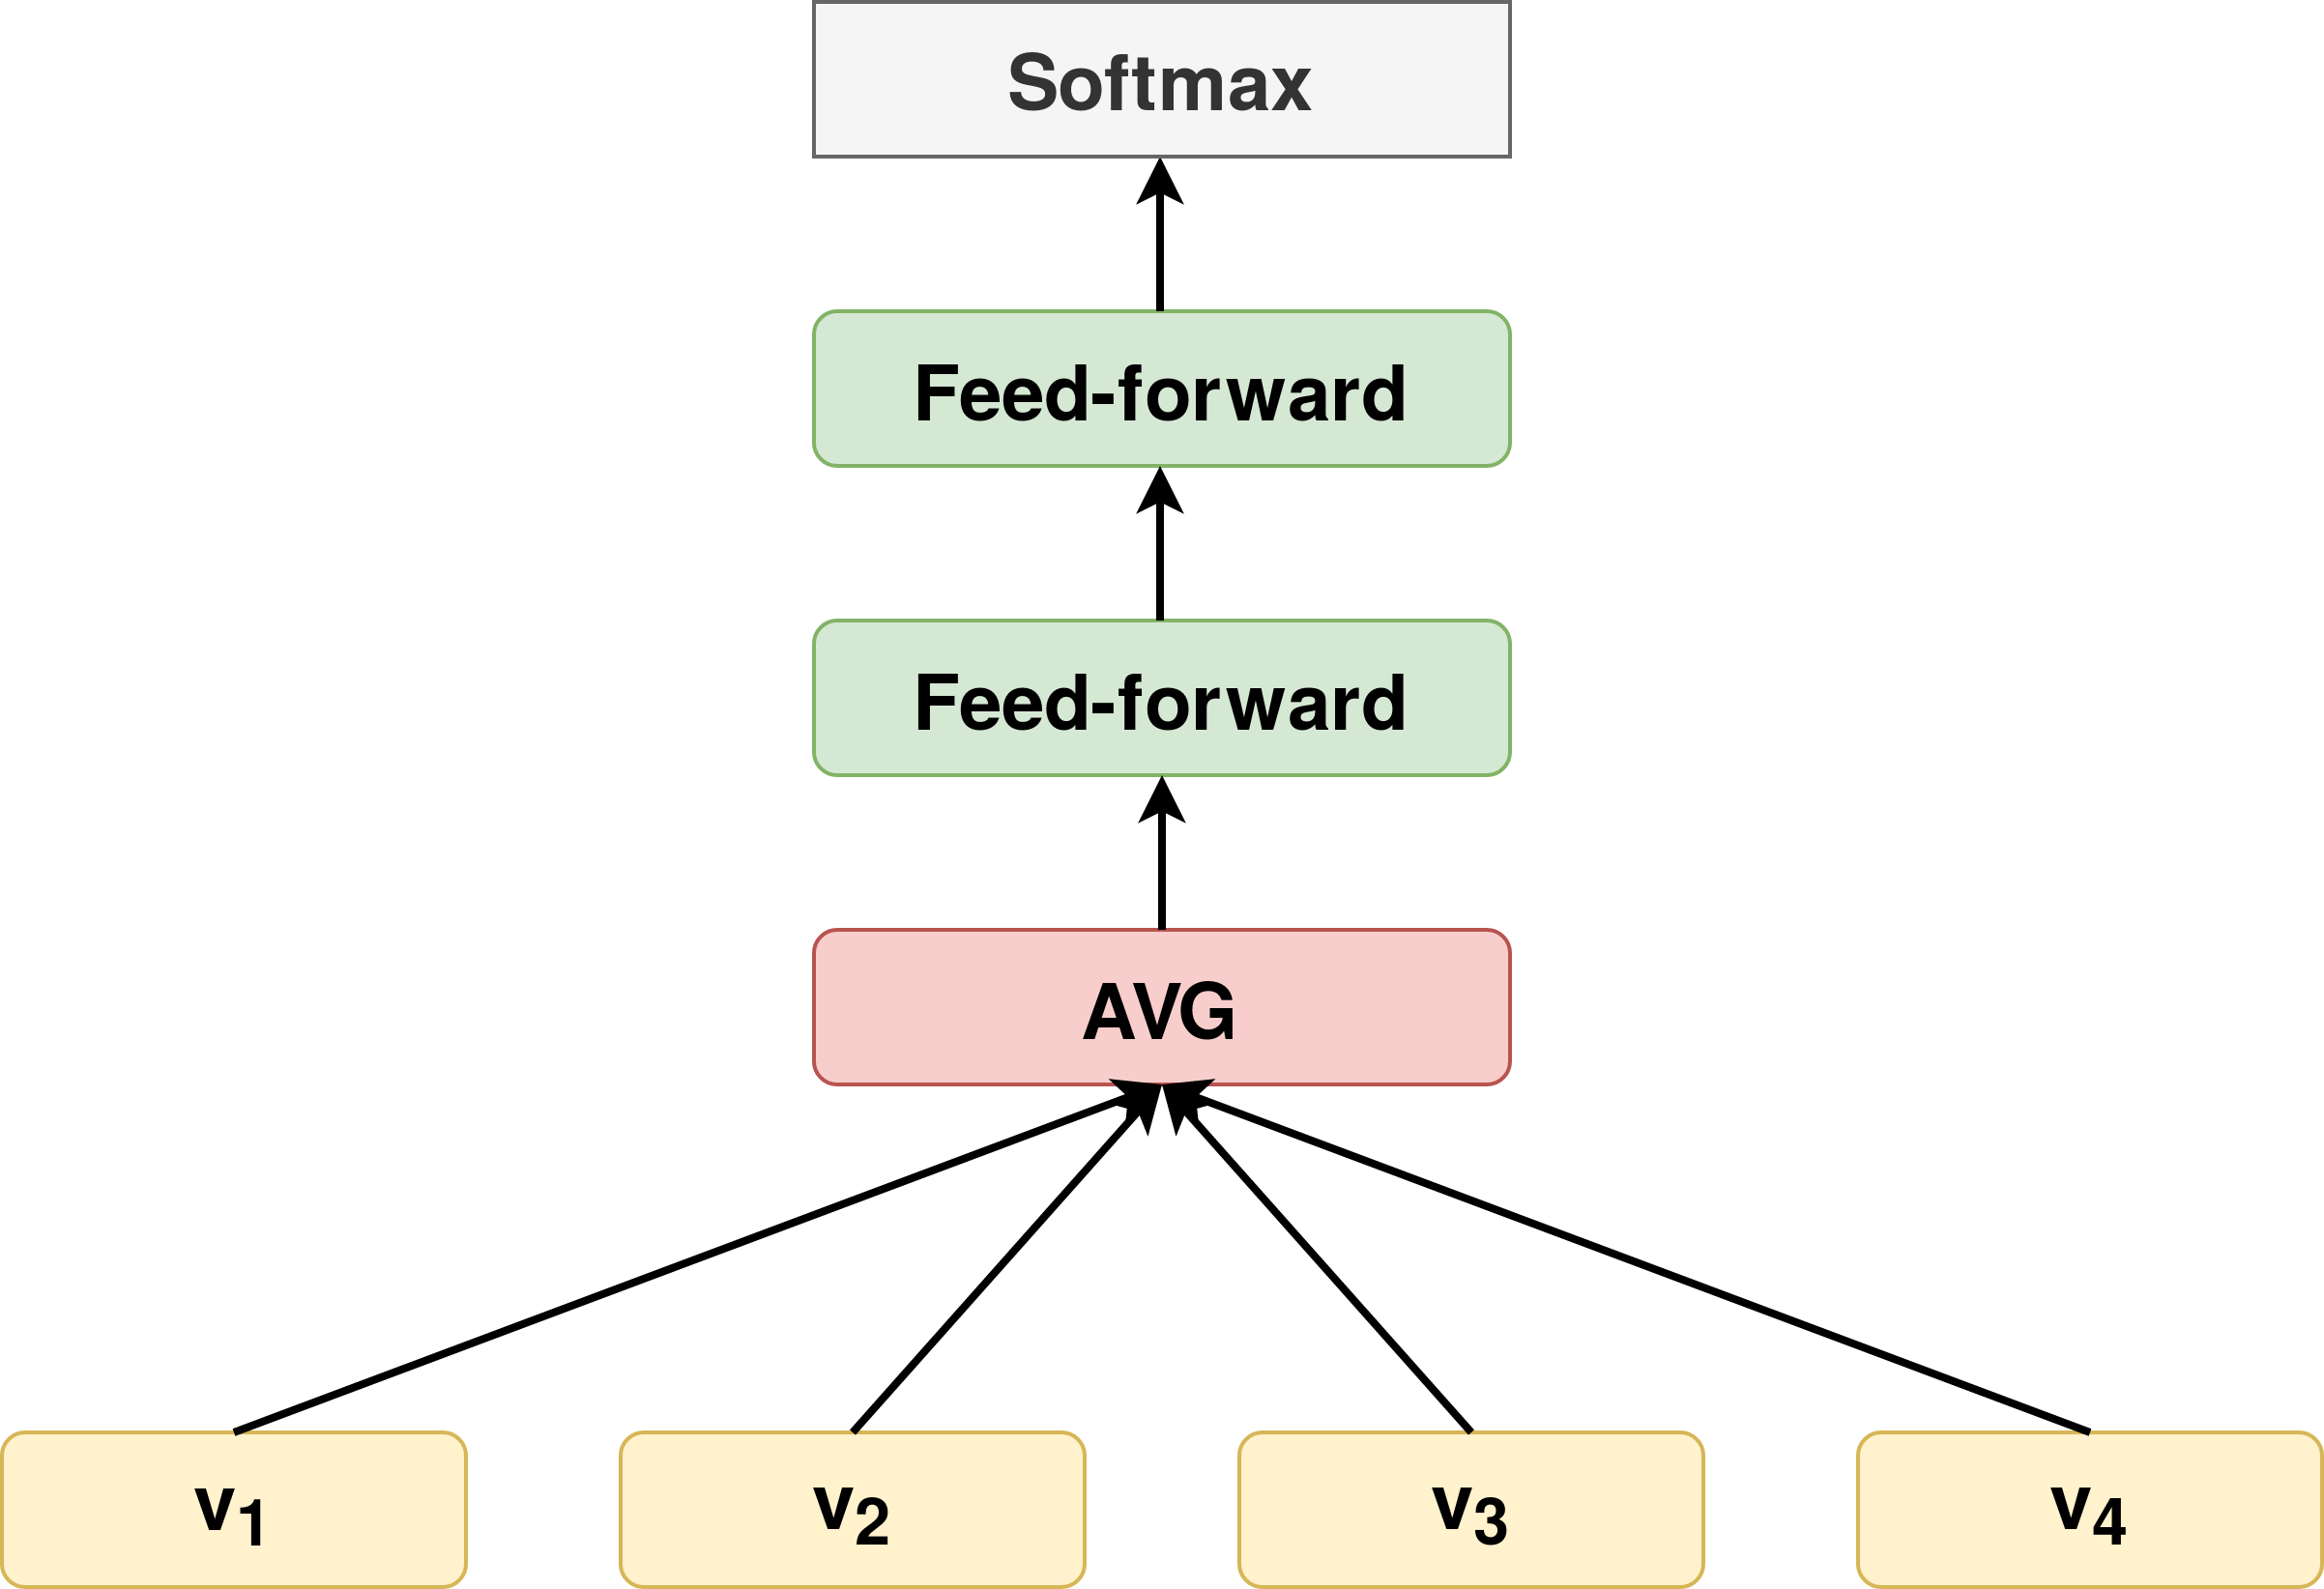
\includegraphics[width=0.6\textwidth,height=150px]{DAN}
	\caption{DAN architektúra}
\end{figure}

A \textit{transformer} modell egyik algráfja a mondatokban lévő szavak kontextusfüggő reprezentációját állítja elő. A folyamat során figyelembe veszi az egyes lexémák sorrendi és egyéni információit is, majd összegzi őket, így megkapja a végső mondatszintű reprezentációt.
A \textit{DAN} modell az input tokenek vektorait először átlagolja, majd \textit{feed forward} rétegek segítségével előállítja a mondatvektorokat. A USE szavakból, mondatokból, vagy akár rövidebb bekezdésekből is képes 512 méretű vektorokat generálni.

A neurális hálók tanítását két részre bontották, bemenetként angol nyelvű karakterláncokat kaptak. Az első rész a \textit{Skip-thought}-hoz hasonló módon, dialógusokból vett mondat-válasz párokkal, illetve felügyelt módon a \textit{Stanford Natural Language Inference} (SNLI) korpuszon történt.

A cikk során kiemelt szerepet kapott a tanítás második fázisa. Számos módon finomhangolták a modelleket és mérték a teljesítményüket. A feladatok közé tartozott, hogy filmes értékelések szövege alapján ki kellett találnia a neurális hálóknak az értékelések pontszámát 1 és 5 között. Továbbá vásárlói értékelések hangulati töltetét kellett prediktálniuk.

 Az algoritmusokat kipróbálták a szavak szintjén, a mondatok szintjén és a kettő módszer konkatenációjaként is. A legjobb teljesítményt a mondatszintű reprezentációk mutatták. A transformer architektúra pontosabb eredményt hozott, mint a DAN alapú modell, de a transformer modell $\mathcal{O}(n^2)$, míg a DAN modell $\mathcal{O}(n)$ időkomplexitású a bemeneti hossz függvényében. Továbbá memóriahasználatban is kedvezőbb választás a DAN.

A \textit{GloVe}-hoz hasonlóan a USE is képes asszociációkra, de jóval gyengébb ezen képessége az olyan kényes témák esetében, mint a szexizmus és a rasszizmus. Ez a tény alkalmassá teheti a USE-t az ipari használatra is.

A szerzők rávilágítottak arra, hogy kevés adat esetén jó választás lehet a \textit{transfer learning} módszere, és a magasabb szintű reprezentációk pontosabb eredményt érhetnek el a legtöbb feladat esetében.

\subsection{Dokumentumszintű reprezentáció}
Ahogy a technológia fejlődik, úgy növekszik a világon az egységnyi idő alatt előállított információ mennyisége is. Gyakori eset, hogy ez írott formában, dokumentumokban jelenik meg. Dokumentumnak tekinthetünk minden, a mondatnál hosszabb emberi nyelven írott szöveget.

Bár a magasabb nyelvi egységek értelmezése és feldolgozása sok területen előkerülő feladat, mégsem triviális. Nagy kihívást jelent a szemantikai szimilaritás mérése, az olyan gyakorlati problémákat nem is említve, mint a duplikációk kiszűrése a fórumokról, vagy a szociális média analízis.

2014-ben a Word2Vec szerzői előálltak egy dokumentumszintű reprezentációs algoritmussal. A Doc2Vec \cite{le2014distributed} módszer a Word2Vec modell kiterjesztése a dokumentumok szintjére. Mivel a dokumentumokat nem lehet a szavakhoz hasonló logikai struktúrába rendezni, ezért a megszokott \textit{CBOW} modell bemeneti vektorai mellé egy speciális, a magasabb nyelvi elem azonosítóját jelölő vektort konkatenáltak. Az algoritmus neve PV-DM. A modell tanítása végén a speciális vektor reprezentációja képviseli a dokumentumot.

\begin{figure}[H]
	\centering
	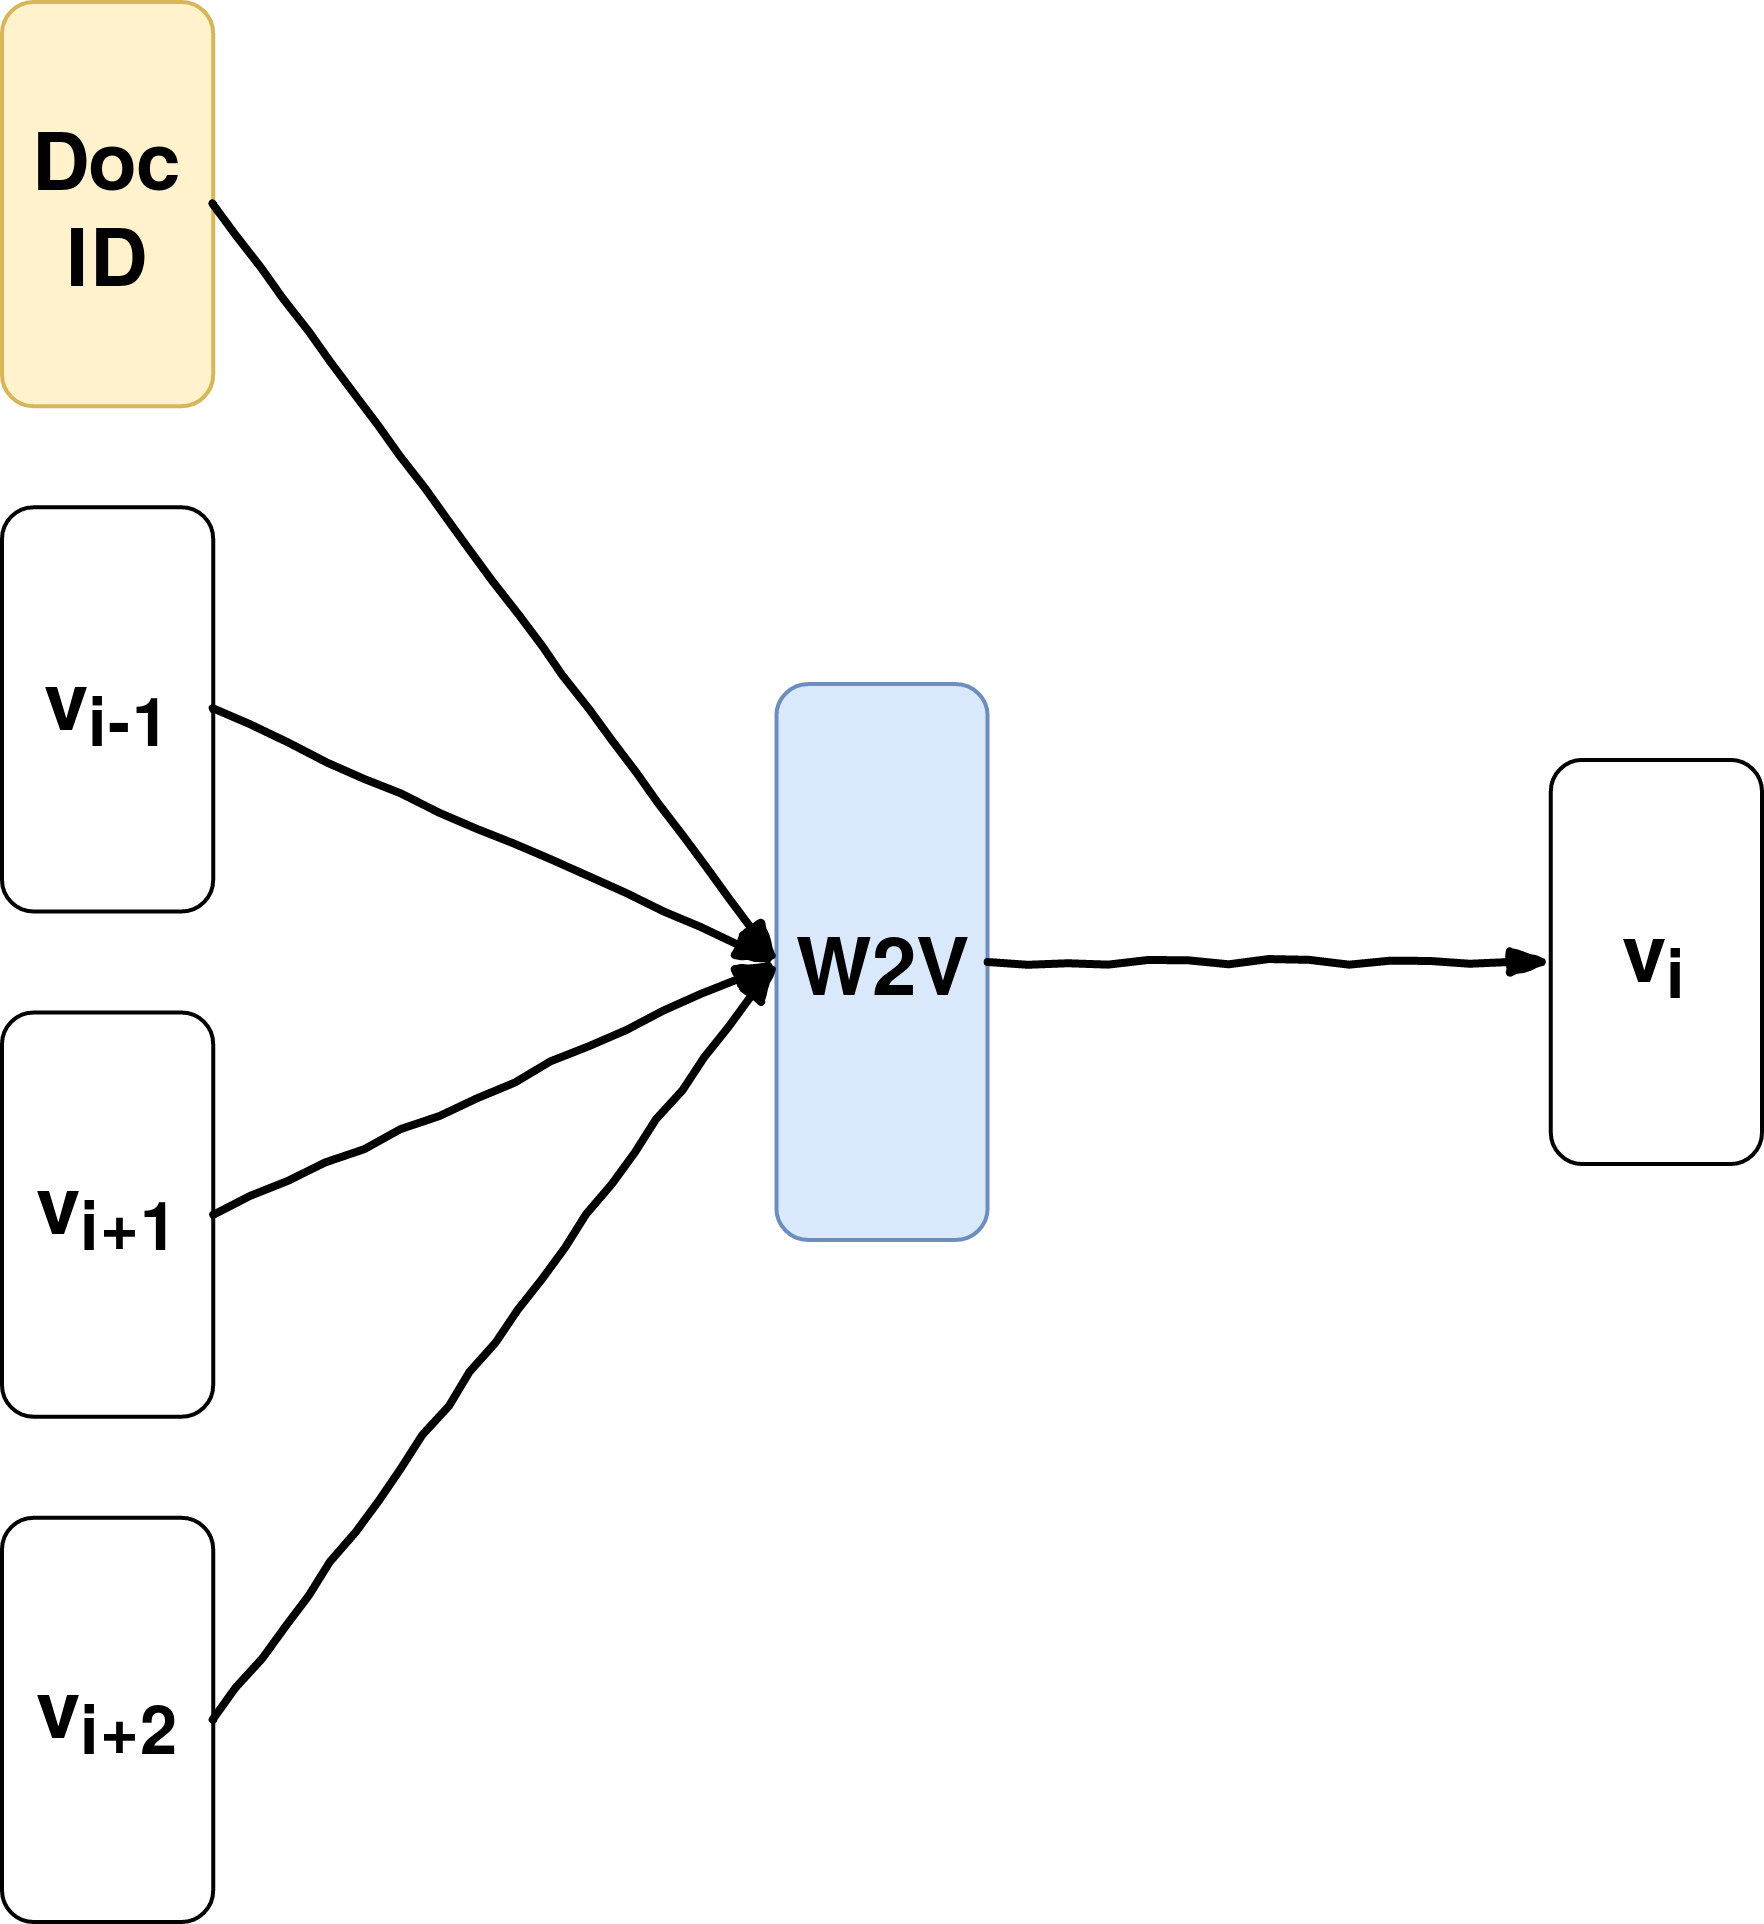
\includegraphics[width=0.5\textwidth,height=150px]{Doc2Vec}
	\caption{Doc2Vec PV-DM architektúra}
\end{figure}

A Word2Vec-hez hasonlóan a Doc2Vec-nek is létezik \textit{Skip-Gram} alternatívája, ez a PV-DBOW. A PV-DBOW modell gyorsabb és memóriahasználat szempontjából is gazdaságosabb a PV-DM-hez képest.

Mivel relatíve kevés algoritmus képes dokumentumszintű modellezésre és azok teljesítménye is limitált, a Doc2Vec egy jó választás lehet. A modell egyszerre mutat jó teljesítményt és a használata is könnyű.

\section{Transfer learning}

A modern szemantikus reprezentációs algoritmusok tanítása összetett folyamat. A feladatok során egyszerre kell több szempontra figyelni, melyek befolyásolhatják a modellünk pontosságát. Példának okáért mondatszintű reprezentációnknak képesnek kell lennie értelmezni a lexémák egymáshoz fűződő viszonyait és a mondatok közötti kohéziót is. A \textit{transfer learning} egy kiváló eszköz arra, hogy modellünket tanítsuk több aspektus szerint.

A \textit{transfer learning} napjainkban közkedvelt tanítási módszer, melynek ötletét az NLP ágazata a számítógépes látás eszközkészletéből merítette. A folyamatot két fázisra lehet bontani: előtanítás és a finomhangolás. Az előtanítás általában nagy mennyiségű adaton történik. A finomhangolás az előtanítás után kapott modell – adott NLP feladathoz szükséges – speciális feladatokon való tanítását jelenti, amely szignifikánsan kevesebb adatot igényel.

\begin{definition}
	Jelölje $D_s$ a forrástartományt, $D_t$ a céltartományt, $T_s$ a forrástartományhoz tartozó feladatot, továbbá $X_t$ és $Y_t$ rendre a $T_t$ célfeladathoz tartozó inputváltozók és  címkék halmazát. A \textbf{transfer learning} célja megtanulni $P(Y_t|X_t)$ feltételes eloszlást $D_t$-ben $D_s$ által gyűjtött információ alapján úgy, hogy $D_s \neq D_t$ vagy $T_s \neq T_t$.	 
\end{definition}

\begin{figure}[H]
	\centering
	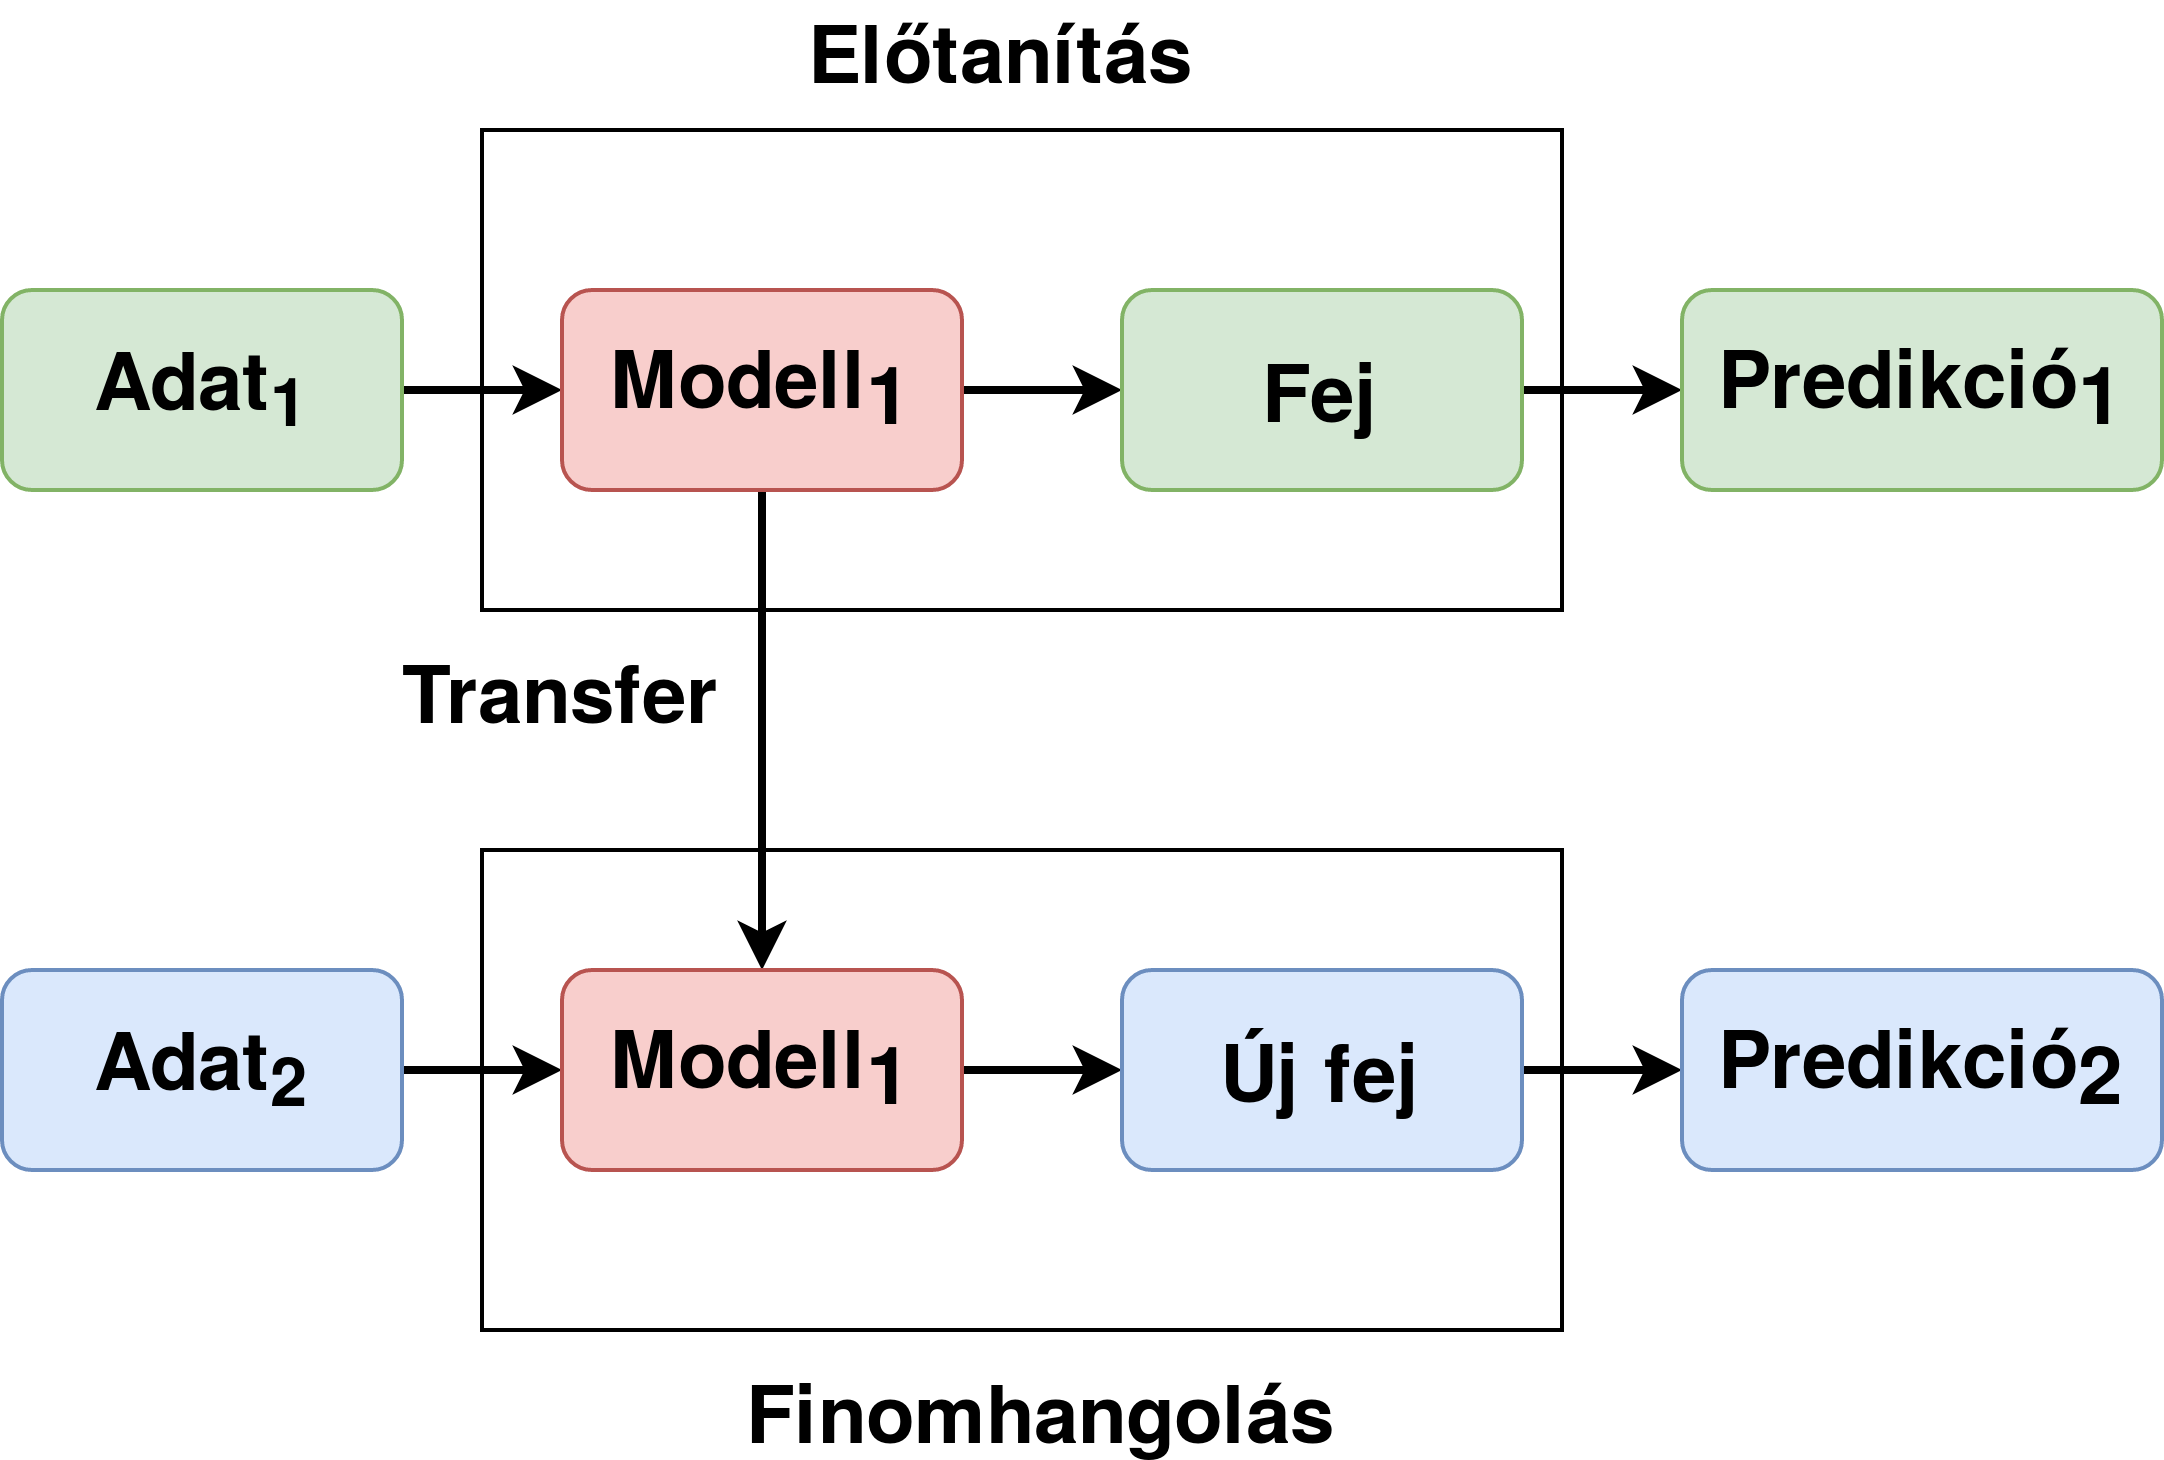
\includegraphics[width=0.6\textwidth,height=170px]{transfer}
	\caption{Transfer learning}
\end{figure}

Az előtanítási szakasz olyan feladattal kezdődik, mely kellőképpen generalizál és a neurális hálónk sok, hasznos és általános információhoz tud jutni. A folyamathoz használt adathalmaz általában nagy mennyiségű annotálatlan adatot tartalmaz, de vannak kivételek, például az InferSent esetében.

A finomhangolási fázis alatt használt feladatok az előtanítás után kapott modell súlyait alkalmazzák, de a bemeneti adatok és a feladatok végrehajtásához szükséges fej lehet eltérő is. Ezen szakasz állhat feladatok sorozatából is, ekkor a súlyokat inkrementálisan használják azok. A sikeres végrehajtást követően modellünk képes lesz komplexebb összefüggések felismerésére és pontosabb eredmény elérésére.

A jelenlegi trendek szerint a reprezentációs módszerek tanítási módja nagyobb hangsúlyt kap, mint maga a neurális háló szerkezete. A \textit{transfer learning} használata a numerikus ábrázolás során még kiaknázatlan terület, mely rendkívül sok eredményt hozhat a jövőben.







